
%%% Local Variables: 
%%% mode: latex
%%% TeX-master: t
%%% End: 

\chapter{环结构特征}
\label{cha:cycle}



本文提出了一种新的局部不变特征,即环结构特征,以应用于图像内容中存在环结构特征的各类图像,比如建筑物图像、树叶图像、视网膜图像、扇贝贝壳图像等。如图\ref{fig:Example}所示,环结构特征由图像中存在的交叉、分叉点及它们之间的连线构成,建筑物中的水泥框架、树叶中的叶脉、视网膜中的血管、扇贝贝壳纹理都可以形成环结构。通过将环结构描述成特征向量,即可应用于识别、配准等各个领域。

\begin{figure}[H]
\centering
  \begin{minipage}[b]{0.48\textwidth} 
      \centering 
      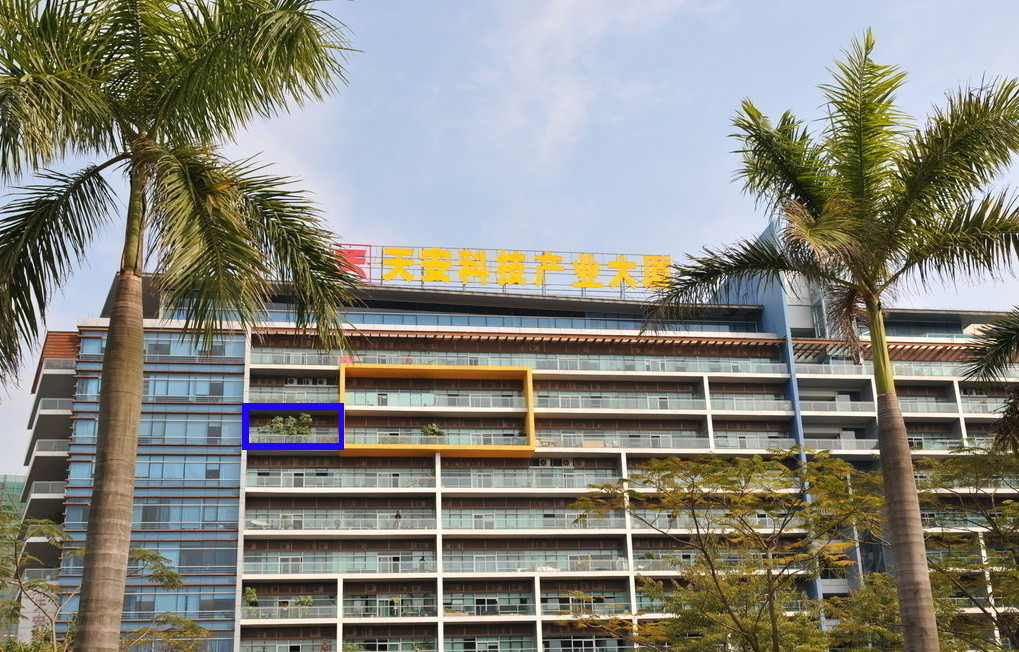
\includegraphics[width=5cm]{chap02/building}
        \centerline{(a) 建筑物}\medskip
    \end{minipage}
  \begin{minipage}[b]{0.48\textwidth}
    \centering
    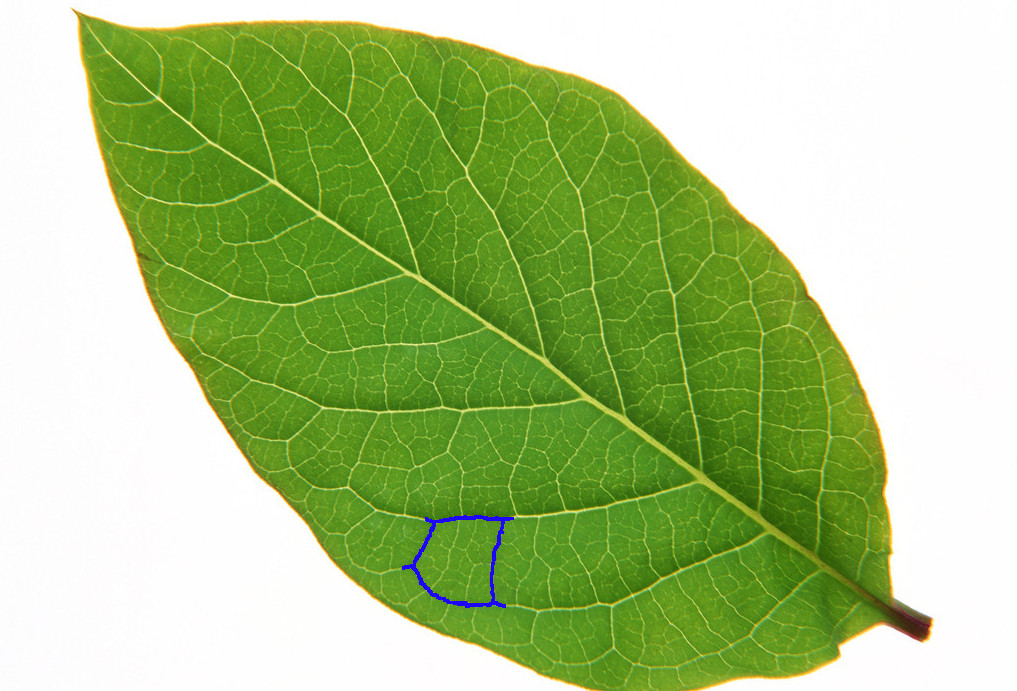
\includegraphics[width=5cm]{chap02/reaf}
      \centerline{(b) 树叶}\medskip
  \end{minipage}
  \begin{minipage}[b]{0.48\textwidth}
    \centering
    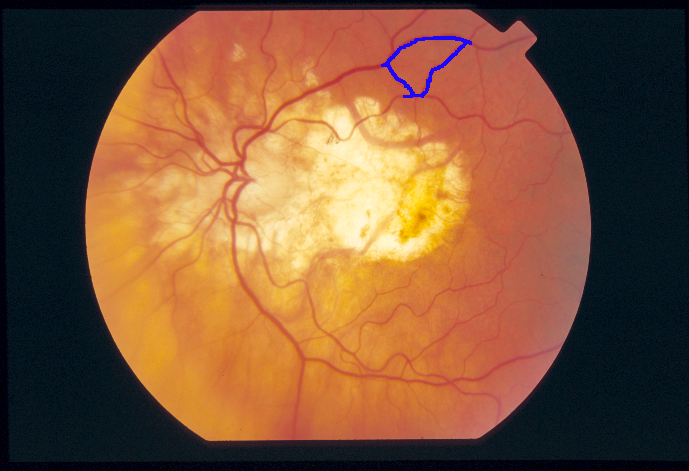
\includegraphics[width=5cm]{chap02/retinal}
      \centerline{(c) 视网膜}\medskip
  \end{minipage}
  \begin{minipage}[b]{0.48\textwidth}
    \centering
    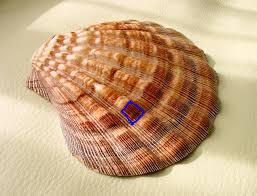
\includegraphics[width=5cm]{chap02/scallop}
      \centerline{(d) 扇贝}\medskip
  \end{minipage}
\caption{图像中的环结构}
\label{fig:Example}
\end{figure}




\section{预处理}
\label{}

原始图像一般都是灰度或彩色图像,若想从中提取环结构来用做识别或配准的特征,需要对其进行预处理,以使得环结构特征更加突出,以便能够准确快速的提取。对于原始图像的预处理主要分为四步,即基于偏微分方程的多尺度图像分割、连通区域标记图像去噪、膨胀腐蚀操作填充孔洞、骨架化,如图\ref{fig:chart-Preprocessing}所示。经过这四步处理,原始图像转化为骨架化后的二值图像,以便进行环结构特征的提取。
\begin{figure}[H]
\centering
    \centering
    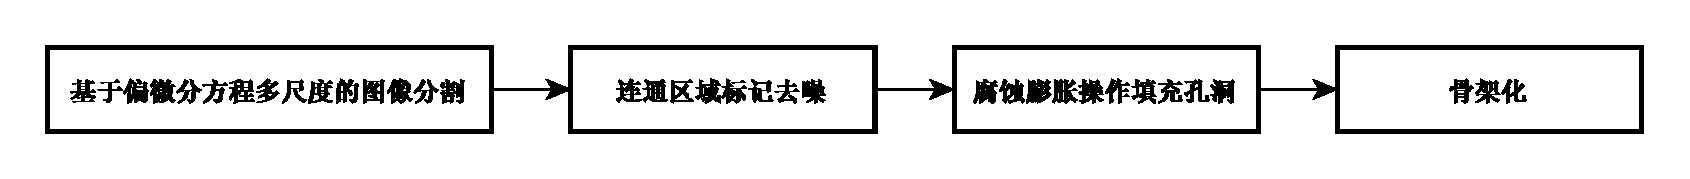
\includegraphics[width=13cm]{chap02/preprocessing}\medskip
\caption{预处理流程图}
\label{fig:chart-Preprocessing}
\end{figure}
\subsection{基于偏微分方程的多尺度图像分割}

图像分割是计算机视觉领域的至关重要的技术,图像分割的结果好坏将很大程度上影响后续对图像的处理及应用。近些年来,对图像分割技术的研究层出不穷,分为基于区域的分割,基于边缘的分割,基于特定理论的分割,如基于模糊理论的分割、基于水平集的分割、基于活动轮廓的分割、基于图论的分割~\cite{xuxiaoli}等等。

环结构特征存在于很多类图像中,不同类图像的环结构之间有很大的不同。例如,视网膜血管图像中血管较细、直径宽度变化范围大,血管与背景对比度低,扇贝贝壳纹理图像中边缘较模糊等,这就增加了图像分割的难度。为了减小图像分割对图像配准或识别的影响,并且使分割结果能够适用于多类不同图像,我们采用了基于偏微分方程多尺度的图像分割。

基于偏微分方程的多尺度图像分割~\cite{wang2013retinal}不需要预处理与训练,可直接用于各类图像的分割。首先,利用多小波核对不同边缘的反映特性的不同,对图像中的边缘进行增强。通过多尺度多层分解方法对归一化的图像进行处理,以达到去除噪声和定位边缘的目的。尺度不同表示边缘的细化程度不同。最后,采用自适应阈值方法得到分割后的二值图像,图\ref{fig:flow-segmentation}为基本流程图。这样一幅图像就得到了不同尺度的多个分割结果,针对不同的应用问题就可以选择不同的尺度进行后续处理。

\begin{figure}[H]
\centering
    \centering
    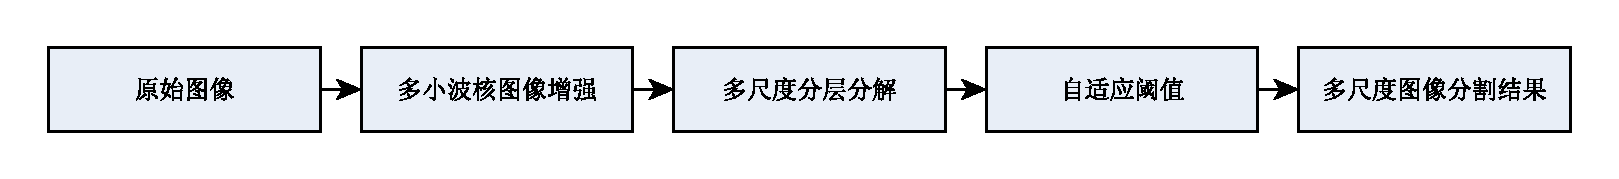
\includegraphics[width=13cm]{chap02/flow-chart-segmentation}\medskip
\caption{多尺度图像分割流程图}
\label{fig:flow-segmentation}
\end{figure}

二维多小波核$ker(x,y;a,b)$可以表示为:
\begin{eqnarray}
k_1(x,y;a,b)&=&\phi_1\{a^{-1}(x-b)\}\\
k_2(x,y;a,b)&=&\phi_2\{a^{-1}(x-b)\}\\
|y| &\geq& L/2
\end{eqnarray}
其中, $(x,y)$,$\phi_i$,$a$,$b$及$L$分别表示像素坐标,一维多小波核尺度函数,尺度参数,平移参数,及二位多小波核在$y$方向的长度。

二维多小波核对二维图像进行匹配滤波实际上就是通过多小波核对图像进行卷积运算的结果,通过对多小波核进行任意角度旋转,然后与图像进行卷积,求最大值,可以得到:
\begin{equation}
M_{ker}(x,y;a,b) = max_\theta(r_\theta(ker(x,y;a,b)) \ast Img(x,y))
\end{equation} 
$r_\theta$表示将多小波核旋转$\theta$角度后得到的结果,$\ast$表示卷积运算。

图像中物体的轮廓或边缘的增强,通过计算多小波核$k_1(x,y;a,b)$与图像最大卷积得到:
\begin{equation}
M_{k_1}(x,y;a,b) = max_\theta(r_\theta(k_1(x,y;a,b)) \ast Img(x,y))
\end{equation} 

多小波核$k_2(x,y;a,b)$与图像局部平均最大卷积可用来增强图像背景:
\begin{eqnarray}
M_{k_2}(x,y;a,b) &=& max_\theta(D_m(r_\theta(k_2(x,y;a,b)) \ast Img(x,y)))\\
D_m(Img) &=& Img\ast W
\end{eqnarray} 
其中,$D_m$表示图像的局部平均,$W$表示一个$w \times w$的滤波器。通过多小波核匹配滤波器的处理,图像中的物体得到增强,并且可与非物体进行区分。

多尺度分层分解是迭代分割的过程,在这个迭代的过程中,越来越多的信息能够被检测到,通过尺度参数可以控制分割的精细程度。

分解模型的数值实现,实质上是最小化欧拉-拉格朗日方程$J(f,\lambda)$的过程:
\begin{equation}
u_\lambda - \frac{1}{2\lambda}div(\frac{\bigtriangledown_{u_\lambda}}{|\bigtriangledown_{u_\lambda}|})
\end{equation}
诺伊曼边界条件为:
\begin{equation}
\frac{\partial_{u_\lambda}}{\partial_n} = 0 \qquad \textrm{on} \qquad \partial \Omega
\end{equation}
其中,$n$是边界$\partial \Omega$的外法线。通过Gauss-Seidel迭代法~\cite{tadmor,nezzar}可以来求解方程。

为了得到二值化的图像分割结果,采用自适应阈值的方法,该方法把边缘的过零点作为插值点得到图像阈值平面。图像的不同区域的二值化阈值不同。通过顺序松弛算法,可以得到$u$的阈值平面$\bar{u}$。则二值化公式为:

\begin{align}
Out(x,y) = \left\{ \begin{array}{ll}
1 & \bar{u}(x,y)\leq u(x,y)\\
0 & \textrm{其他}
\end{array} \right.
\end{align}
Out为最终得到的二值化图像。

图\ref{fig:Segmentaion-retinal}显示了视网膜图像的三个不同尺度的分割结果,图a为原图,b、c、d分别为不同尺度的分割结果。从图中可以看出,从图b到图d,越来越多的血管被分割出来。b图中只分割出了原图中较为粗的血管,图d分割出了更为精细的血管。但从d图中可以看出分割的越精细,噪声也越大。图\ref{fig:Segmentaion-retinal1}是一组树叶图像的例子。可以很明显地看出从图b到图d,图像的细节信息越来越多地被分割出来。通过多尺度分割算法,可以得到图像不同层面的信息,这样,针对不同种类的图像的应用问题,就可以选择合适的分割尺度得到最佳的分割结果。

\begin{figure}
\centering
  \begin{minipage}[b]{0.48\textwidth} 
      \centering 
      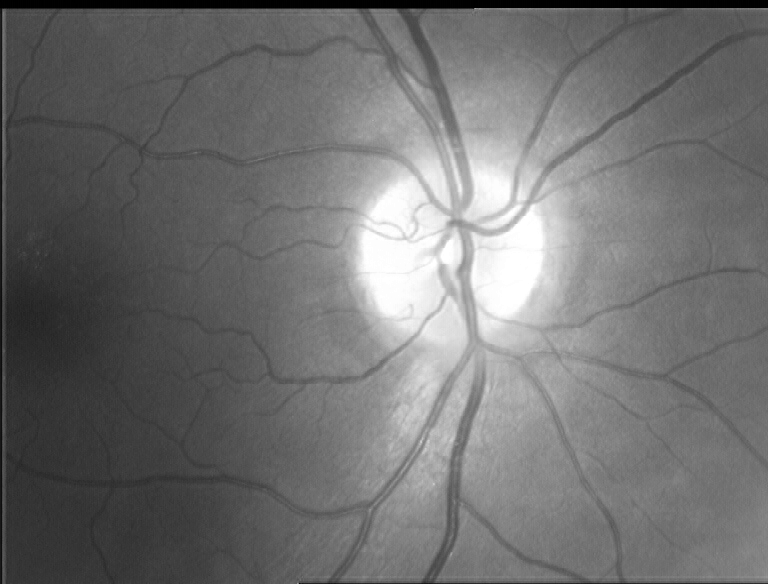
\includegraphics[width=6cm]{chap02/118}
        \centerline{(a)}\medskip
  \label{Segmentaion-retinal:a}
    \end{minipage}
  \begin{minipage}[b]{0.48\textwidth}
    \centering
    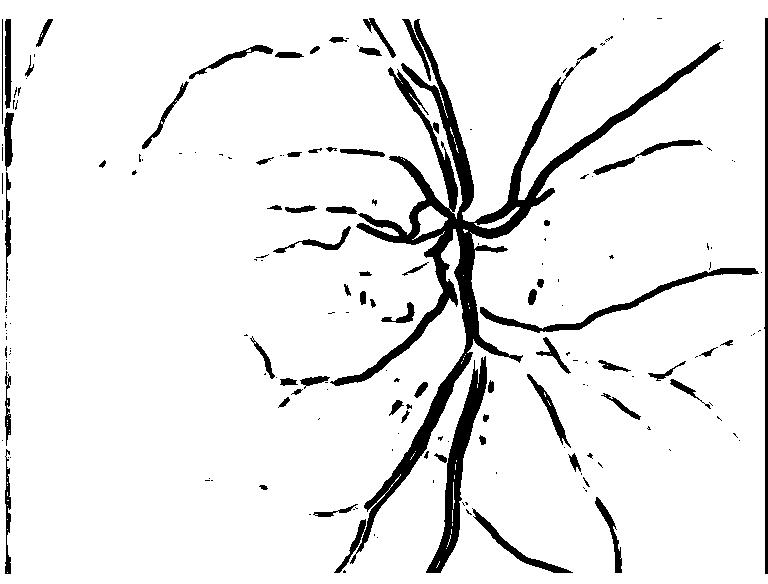
\includegraphics[width=6cm]{chap02/118-13}
      \centerline{(b)}\medskip
   \label{Segmentaion-retinal:b}
  \end{minipage}
  \begin{minipage}[b]{0.48\textwidth}
    \centering
    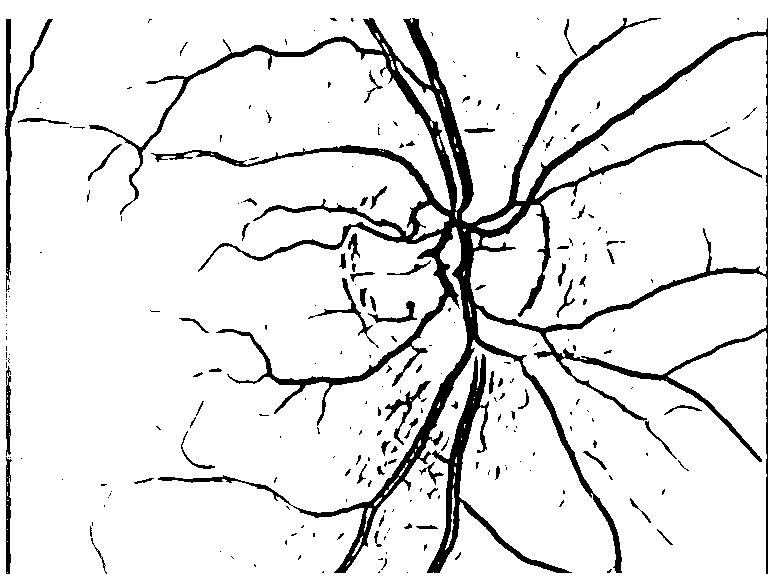
\includegraphics[width=6cm]{chap02/118-08}
      \centerline{(c)}\medskip
     \label{Segmentaion-retinal:c}
  \end{minipage}
  \begin{minipage}[b]{0.48\textwidth}
    \centering
    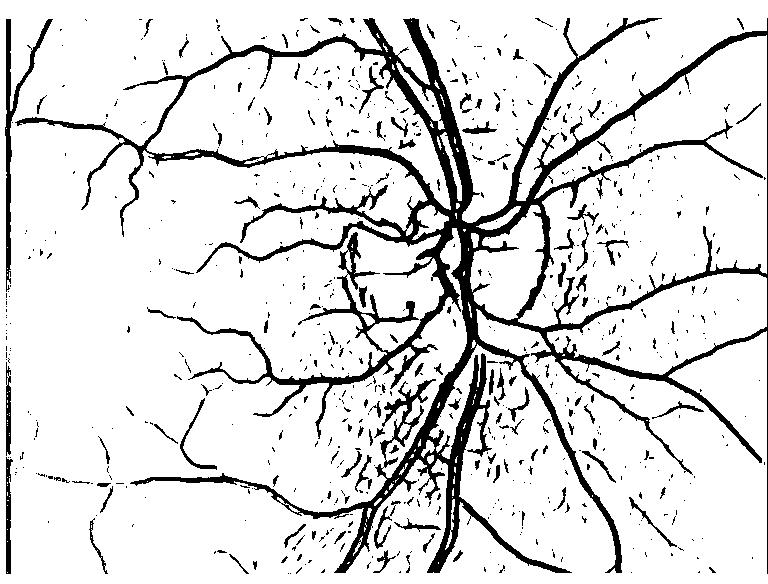
\includegraphics[width=6cm]{chap02/118-01}
      \centerline{(d)}\medskip
	   \label{Segmentaion-retinal:d}
  \end{minipage}
\caption{不同尺度的视网膜图像分割结果。a为原图,b、c、d分别代表不同尺度的分割结果。}
\label{fig:Segmentaion-retinal}
\end{figure}

\begin{figure}
\centering
  \begin{minipage}[b]{0.48\textwidth} 
      \centering 
      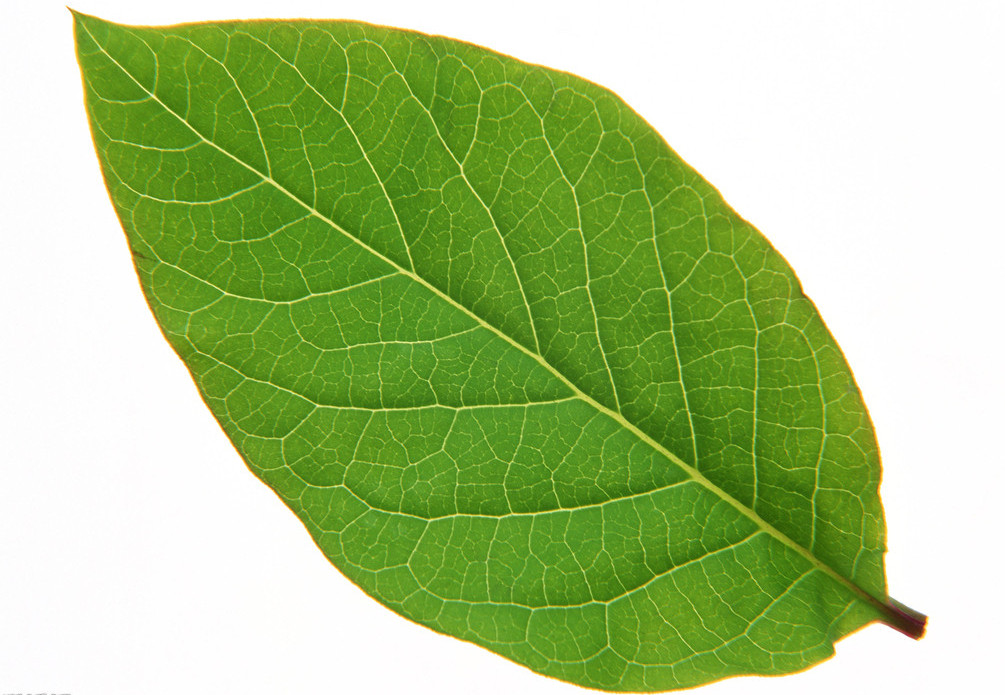
\includegraphics[width=6cm]{chap02/reaf-origin}
        \centerline{(a)}\medskip
    \end{minipage}
  \begin{minipage}[b]{0.48\textwidth}
    \centering
    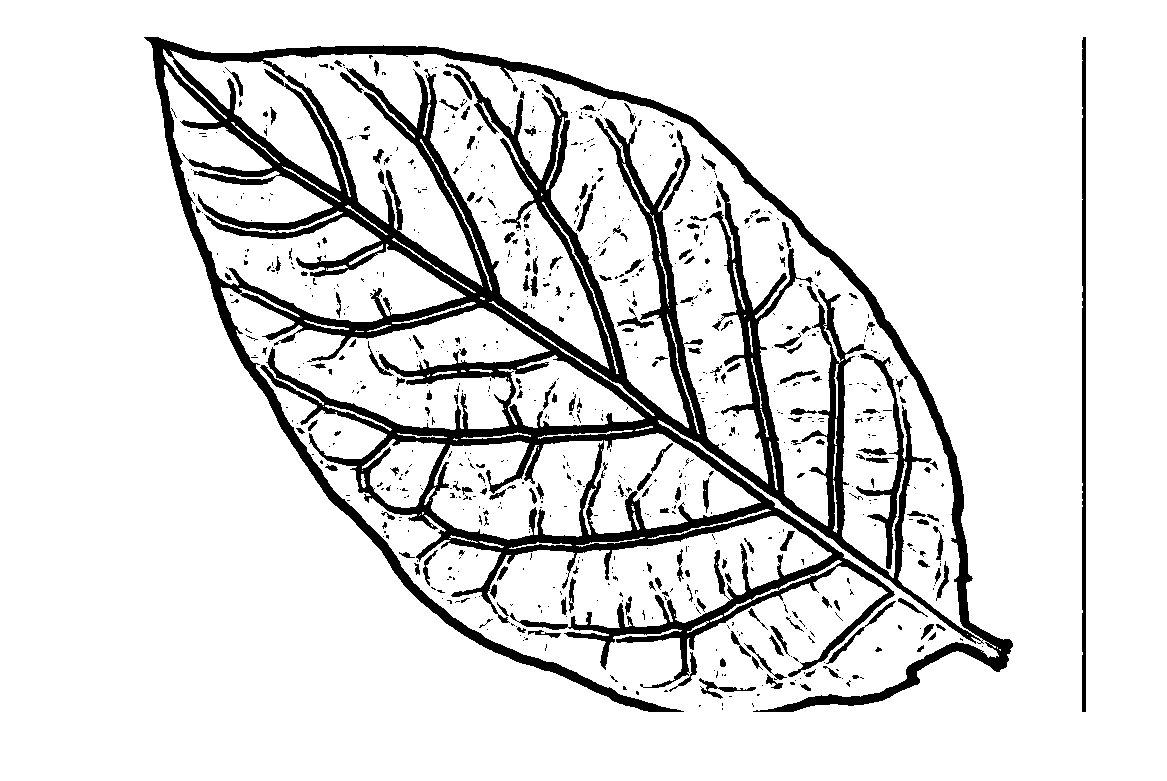
\includegraphics[width=6cm]{chap02/reaf1}
      \centerline{(b)}\medskip
  \end{minipage}
  \begin{minipage}[b]{0.48\textwidth}
    \centering
    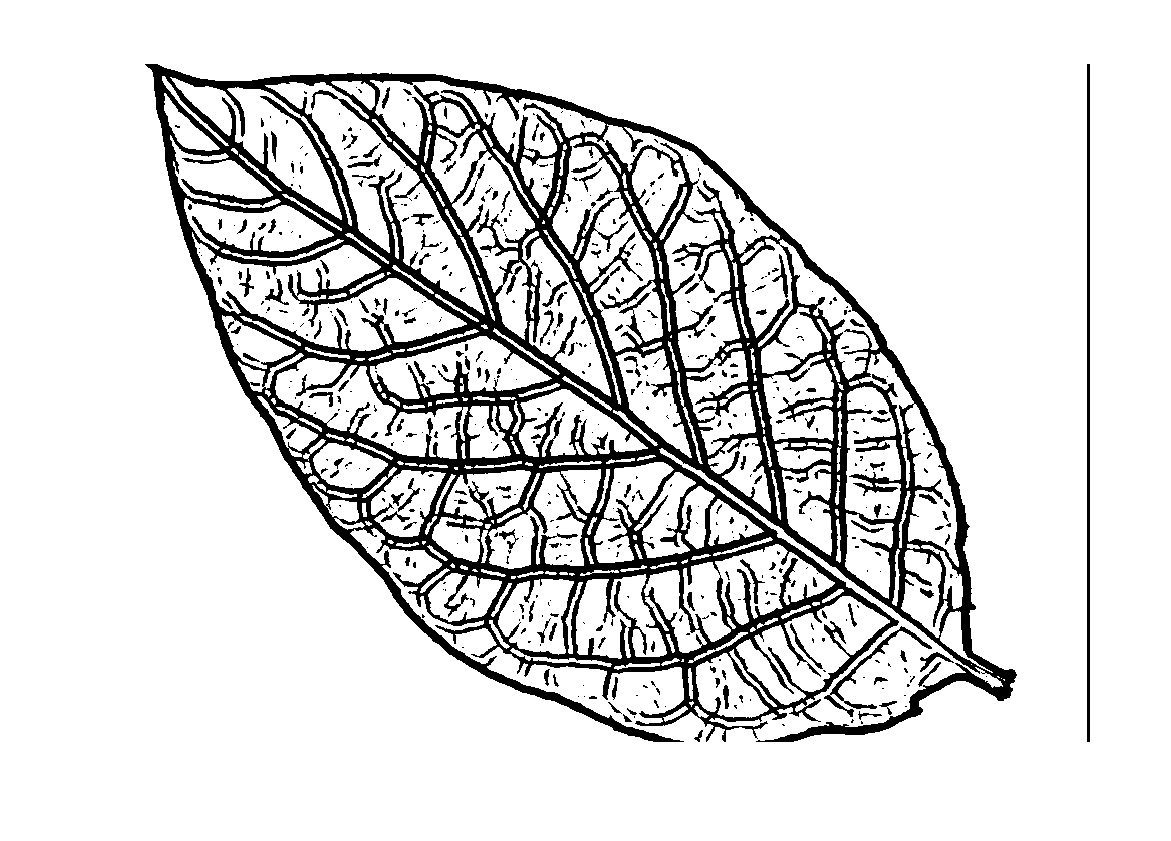
\includegraphics[width=6cm]{chap02/reaf3}
      \centerline{(c)}\medskip
  \end{minipage}
  \begin{minipage}[b]{0.48\textwidth}
    \centering
    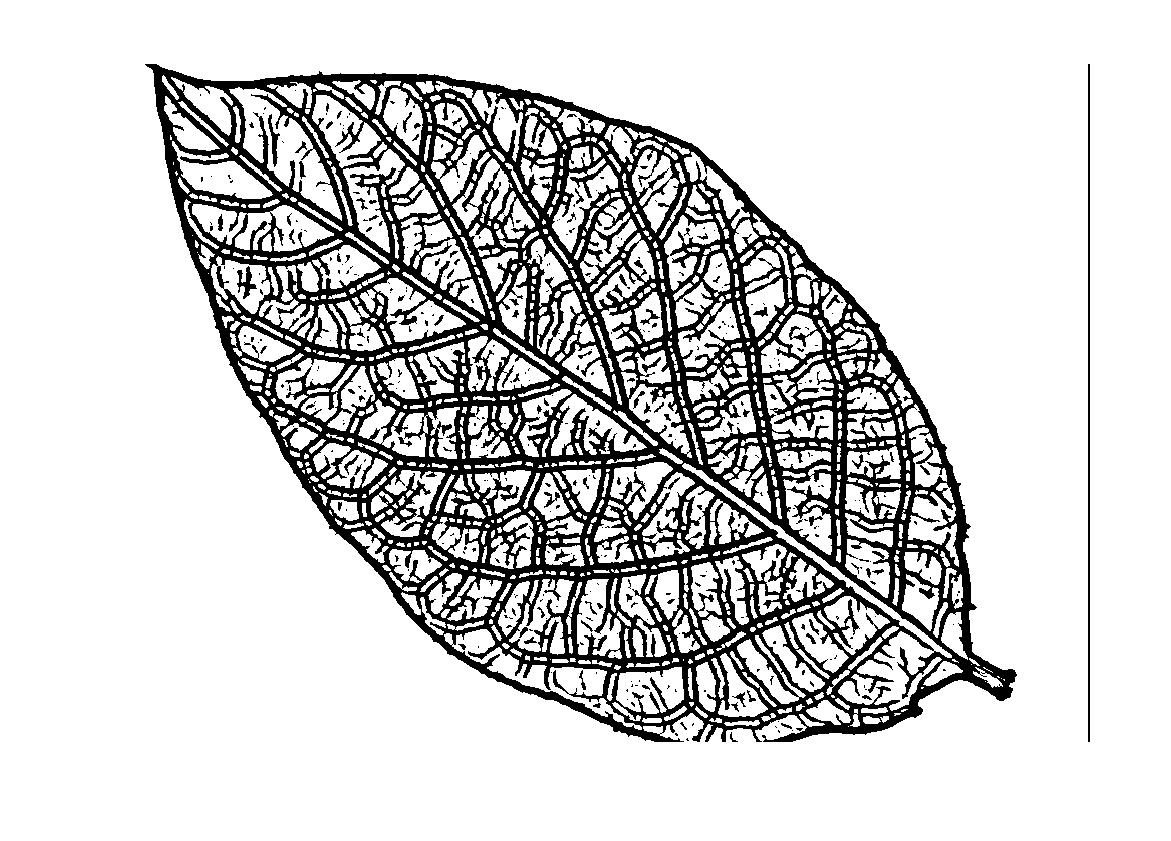
\includegraphics[width=6cm]{chap02/reaf2}
      \centerline{(d)}\medskip
	\label{fig:max}
  \end{minipage}
\caption{不同尺度的树叶图像分割结果。a为原图,b、c、d分别代表不同尺度的分割结果}
\label{fig:Segmentaion-retinal1}
\end{figure}

然而,若原图亮度不均或背景中存在较大噪声,分割尺度较大时虽然会把图像的细节分割出来,但噪声也会随之被分割出来,这样就增加环结构提取的困难度。为了消除噪声对环结构提取的影响,要对分割后的图像进行去噪处理。

\subsection{连通区域标记图像去噪}

连通区域标记~\cite{xuzhengguang}是图像处理中常用的一个基本方法,在目标分割、边缘检测中有着十分广泛的应用。同时,连通区域也可应用于图像去噪。
采用连通区域算法对连通区域进行标记,即通过对二值图像进行逐行逐列扫描,根据图像中像素之间的邻域关系,对属于同一四连通或八连通区域的像素赋予相同的标号,然后统计同一标号的像素的个数。若像素数小于某个阈值,则认为是噪声。

邻域关系有两种,即四邻域与八邻域。设像素$P(x, y)$,则像素$P$的四邻域表示为$P_1(x,y-1)$、$P_2(x, y+1)$、$P_3(x-1,y)$、$P_4(x+1,y)$,像素$P$的八邻域表示为$P_1(x,y-1)$、$P_2(x, y+1)$、$P_3(x-1,y)$、$P_4(x+1,y)$、$P_5(x-1,y-1)$、$P_6(x+1, y+1)$、$P_7(x-1,y+1)$、$P_8(x+1, y-1)$,更加直观的表示如表\ref{tab:adjacent}。为了更好的去除噪声,我们采用八邻域去噪。
\begin{table}[H]
\centering
\caption{四邻域与八邻域}
\begin{tabular}{|c|c|c|}
\hline
 & $P_1$ & \\
\hline            
$P_3$ & $P$ & $P_4$\\
\hline           
& $P_2$ & \\
\hline
\end{tabular}
\begin{tabular}{|c|c|c|}
\hline
$P_5$ & $P_1$ & $P_7$\\
\hline            
$P_3$ & $P$ & $P_4$\\
\hline            
$P_8$& $P_2$ & $P_6$ \\
\hline
\end{tabular}

\label{tab:adjacent}
\end{table}


图\ref{fig:denoise-table}是一幅二值图像的连通区域标记图,从图中可以看出,共有$2$个连通区域,标号为$1$、$2$。其中连通区域1只有两个像素,连通区域$2$有$11$个像素,若设定$10$个像素为基准,小于$10$个像素的连通区域为噪声,则连通区域$1$将被认为是噪声,进行去除,而连通区域$2$将被保留。\ref{fig:Preprocessing}(b)是图\ref{fig:Preprocessing}(a)经过去噪后的结果,从图中可以看出很多的噪声都被滤除了。这一步骤不仅会减小环提取过程的复杂性,也避免了噪声形成的假环结构被提取出来的情况。


\begin{figure}[H] % use float package if you want it here
  \centering
  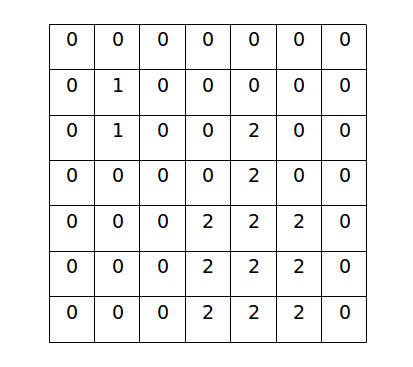
\includegraphics[width=0.4\textwidth]{chap02/denoise-table}
  \caption{连通区域标记去噪。区域1只有两个像素,若设置10个像素为阈值,则1被认为是噪声,需被去除。}
  \label{fig:denoise-table}
\end{figure}



\subsection{膨胀腐蚀操作填充孔洞}
在有些情况下,有时图像的亮度值不均匀,这就造成了分割出的线是断裂的或有孔洞的情况,为了骨架化后的图像能准确的体现原图像的特征,需对分割后的图像进行先膨胀后腐蚀操作。
膨胀腐蚀是图像形态学中比较常见的处理,一般是对二值图像进行处理。
用$b$对函数$f$进行的灰度膨胀~\cite{gang}表示为:
\begin{align}
(f\oplus b)(s,t)=max\{f(s-x, t-y)+b(x,y)|(s-x),(t-y)\in D_f;(x,y)\in D_b\}
\end{align}
其中,$D_f$和$D_b$分别是$f$和$b$的定义域。
灰度腐蚀表示为$f \ominus b$,定义为:
\begin{align}
(f \ominus b)(s,t)=min\{f(s+x, t+y)-b(x,y)|(s+x),(t+y)\in D_f;(x,y)\in D_b\}
\end{align}

图\ref{fig:peng-fu}显示了先膨胀后腐蚀与先腐蚀后膨胀的区别。a、d为原图,三个黑色矩形块之间的两个空隙分别为$5$个与$10$个像素,若采用$5\times5$的矩形窗口对图像进行膨胀腐蚀与腐蚀膨胀操作,得到的最终结果如图c与f。从图中可以看到,先膨胀后腐蚀后,狭窄的缝隙被填充了,而在此例中先腐蚀后膨胀后得到的结果与原图相同。视网膜图像的示例如图\ref{fig:Preprocessing}(c)所示,血管中心位置的孔洞被成功填充。

\begin{figure}
\centering
  \begin{minipage}[b]{0.3\textwidth} 
      \centering 
      
\includegraphics[width=6cm]{chap02/peng-origin}
        \centerline{(a)原图}\medskip
    \end{minipage}
  \begin{minipage}[b]{0.3\textwidth}
    \centering
    
\includegraphics[width=6cm]{chap02/peng-fu}
      \centerline{(b)膨胀}\medskip
  \end{minipage}
  \begin{minipage}[b]{0.3\textwidth}
    \centering
    
\includegraphics[width=6cm]{chap02/peng-fu}
      \centerline{(c)膨胀后腐蚀}\medskip
  \end{minipage}
   \begin{minipage}[b]{0.3\textwidth} 
      \centering 
      
\includegraphics[width=6cm]{chap02/peng-origin}
        \centerline{(d)原图}\medskip
    \end{minipage}
  \begin{minipage}[b]{0.3\textwidth}
    \centering
    
\includegraphics[width=6cm]{chap02/fu-peng1}
      \centerline{(e)腐蚀}\medskip
  \end{minipage}
  \begin{minipage}[b]{0.3\textwidth}
    \centering
    
\includegraphics[width=6cm]{chap02/fu-peng2}
      \centerline{(f)腐蚀后膨胀}\medskip
  \end{minipage}
\caption{先膨胀后腐蚀与先腐蚀后膨胀}
\label{fig:peng-fu}
\end{figure}

\subsection{骨架化}
为了获得一个像素宽的骨架化结果,我们采用轮廓修剪骨架提取方法~\footnote{\url{http://www.cs.smith.edu/~nhowe/research/code/}}。这个方法是Nicholas R. Howe实现的,想法是Alex Telea提出的。若一个点位于一个圆圈的中心,并接触一个图像边缘的多个点,灰度骨架化图像的强度是基于围绕图像的周长连接最远的两点的最短距离。因此,骨架中的毛刺是由微小的边缘扰动引起的强度变化。如果圆圈接触断裂的边缘,骨架化将会是无限的过程。最终的骨架化结果是通过噪声突起轮廓的预期大小来确定的阈值来决定的。图\ref{fig:Preprocessing}(d)是骨架化结果,从图中可以看到,骨架后的图像能准确的描绘出血管的主轮廓。
\begin{figure}[H]
\centering
  \begin{minipage}[b]{0.48\textwidth}
    \centering
    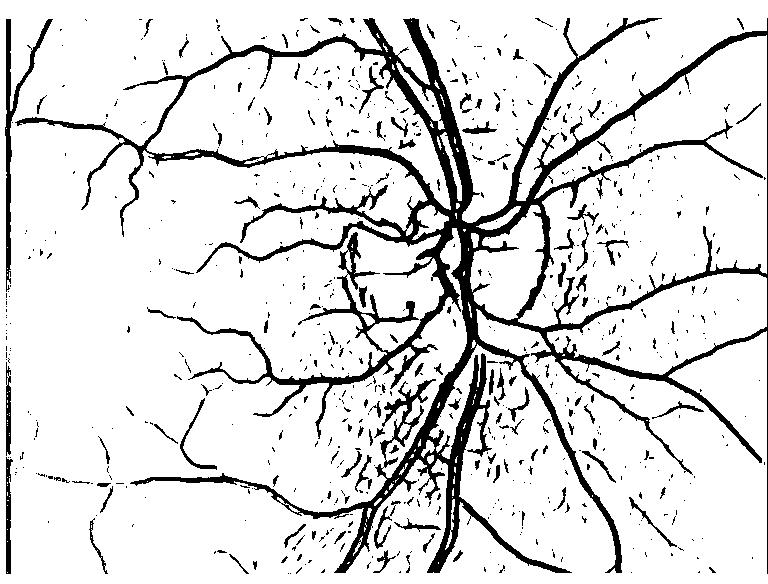
\includegraphics[width=6cm]{chap02/118-01}
      \centerline{(a) 分割图}\medskip
  \end{minipage}
  \begin{minipage}[b]{0.48\textwidth}
    \centering
    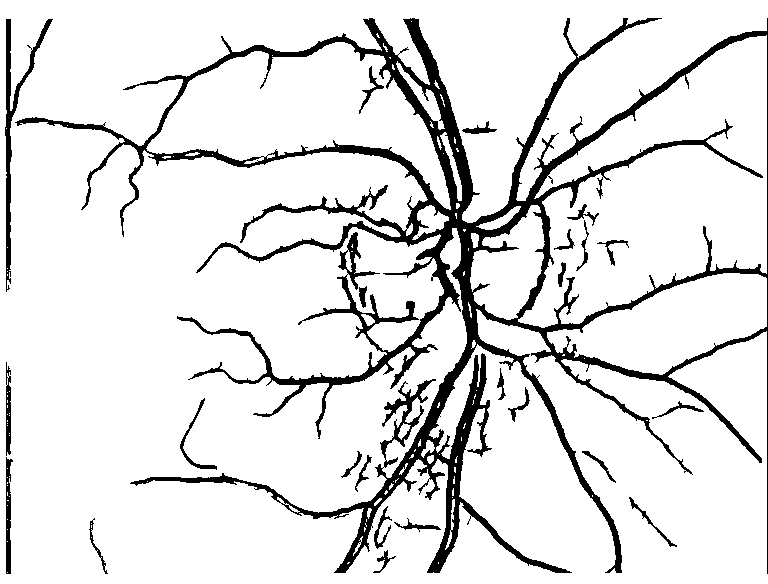
\includegraphics[width=6cm]{chap02/denoise}
      \centerline{(b) 去噪图}\medskip
  \end{minipage}
  \begin{minipage}[b]{0.48\textwidth}
    \centering
    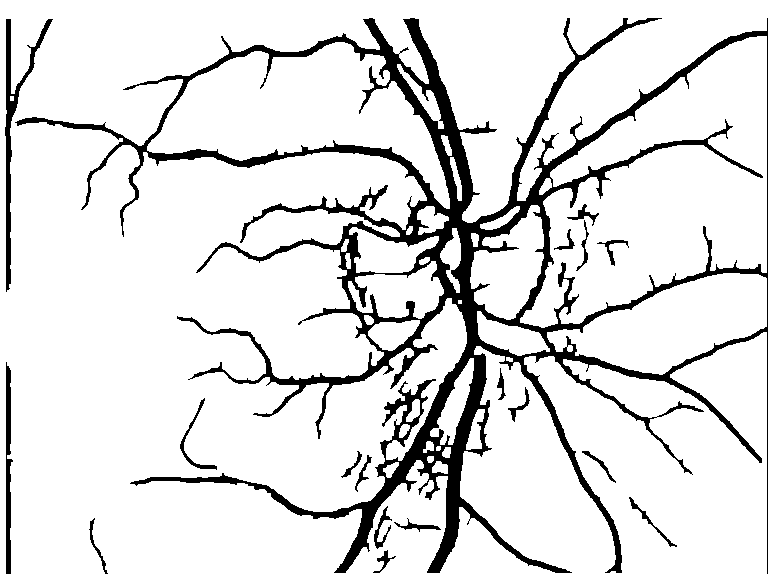
\includegraphics[width=6cm]{chap02/fill}
      \centerline{(c) 填充图}\medskip
  \end{minipage}
  \begin{minipage}[b]{0.48\textwidth}
    \centering
    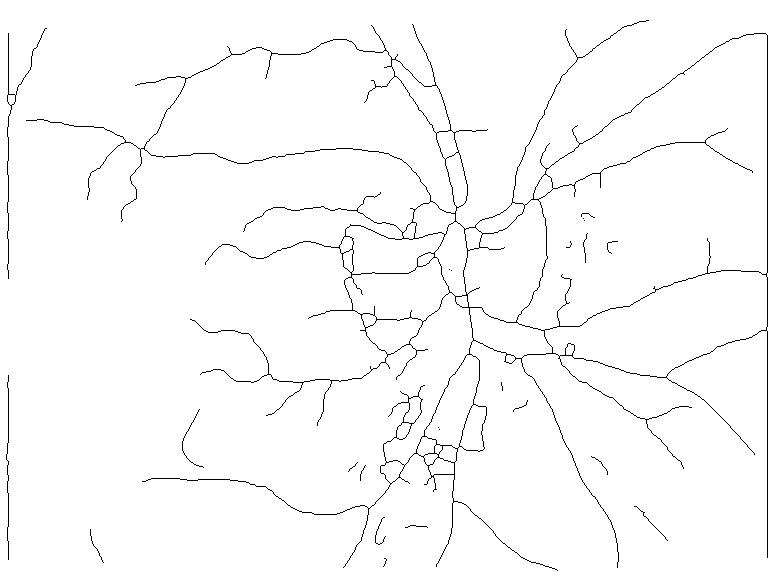
\includegraphics[width=6cm]{chap02/118-skel}
      \centerline{(d) 骨架图}\medskip
  \end{minipage}
\caption{预处理}
\label{fig:Preprocessing}
\end{figure}

经过这四个步骤,各类彩色图像就变为去噪后的骨架化二值图像,其中的环结构具有一个像素宽度,这样就为检测环结构做好了准备。

\section{环结构检测}
\label{}
\subsection{图论相关概念}
\label{}

图像中环的概念是由图论扩展而来的。在人类社会的实际生活中,有时在描述某些事物或对象之间有某种特定关系时采用图形的方式显得更加直观。对象用图形中的点表示,两对象之间具有的某种特定的关系用两点之间的无向或有向连线表示,由此数学抽象产成了图的概念。

\begin{definition}
一个图$G$定义为一个数学结构$(V, E, \phi)$~\cite{xujunming},其中
\begin{enumerate}
\item $V$是一个集合,其中的元素成为顶点;
\item $E$是定义在$V$上的可以重复的二元关系集,其中的元素成为边;
\item $\phi$ 是$E$到$V$的一个映射。 
\end{enumerate}
若$\phi(E)$中的元素全是有序对,则$(V, E, \phi)$成为有向图,否则,成为无向图。我们所研究的图像中的线是无方向的,所以我们可以把图像认为是无向图。
\end{definition}

在图像中,顶点可以定义为线的交叉、分叉点或孤立点,边为连接两个顶点的连线,如图\ref{fig:graph}所示,$V = \{v_1, v_2, v_3, v_4, v_5\}$,$E = \{e_1, e_2, e_3, e_4\}$,边$e_1$把顶点$v_1, v_2$连接起来。

\begin{figure}[H] % use float package if you want it here
  \centering
  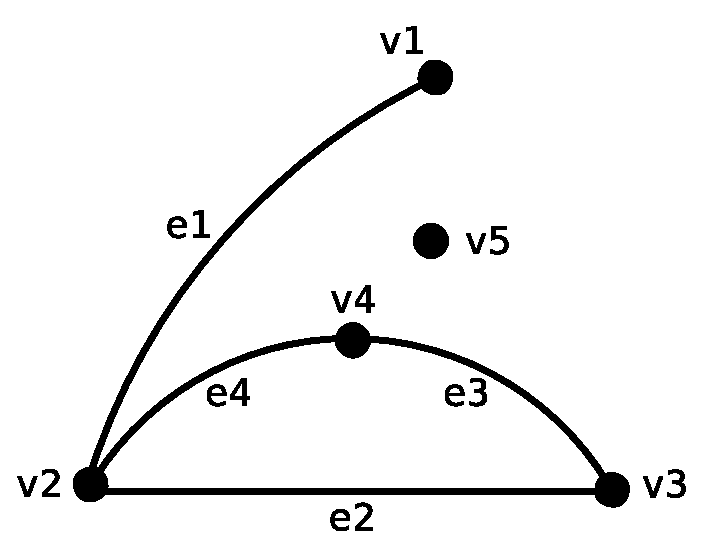
\includegraphics[width=0.3\textwidth]{chap02/graph}
  \caption{图}
  \label{fig:graph}
\end{figure}

\begin{definition}
设$G$是无向图,$x\in V(G)$的顶点度定义为$G$中与$x$关联边的数目,记为$d_{G}(x)$~\cite{wangshuhe}。
\end{definition}

图\ref{fig:graph}中,只有一条边$e_1$与顶点$v_1$相连,即$d_{v_1}=1$,类似的,$d_{v_2}=3, d_{v_5}=0$。


\begin{definition}
设无向图$G = (V, E), v_i, v_j \in V$,若存在一条边$e$以$v_i, v_j$为端点,即$e = (v_i, v_j)$,则称$v_i, v_j$是彼此相邻的,简称相邻的。 
\end{definition}
例如,图\ref{fig:graph}中,$v_1$与$v_2$是相邻的,$v_2$与$v_5$是不相邻的。

设$(V, E, \phi)$是无向图$G$,其中$V = \{v_1, v_2, \ldots, v_p\}$,$E = \{e_1, e_2, \ldots, e_\varepsilon\}$。则无向图$G$的邻接矩阵能够反映出$V$中元素与$E$中元素之间的关联关系。
\begin{definition}
设图$G$的顶点集$V = \{v_1, v_2, \ldots, v_p\}$,令
\begin{align}
a_{ij} = \left\{ \begin{array}{ll}
1 & \textrm{$v_i$与$v_j$相邻}\\
0 & \textrm{$v_i$与$v_j$不相邻或$i = j$}
\end{array} \right.
\end{align}
则称由元素$a_{ij} (i, j == 1, 2, \ldots, p)$构成的$p$阶矩阵为图$G$的邻接矩阵~\cite{wangzhaorui},记作$A$。
\end{definition}
图\ref{fig:graph}的邻接矩阵是
\begin{align}
A = \left( \begin{array}{lllll}
0 & 1 & 0 & 0 & 0 \\
1 & 0 & 1 & 1 & 0 \\
0 & 1 & 0 & 1 & 0 \\
0 & 1 & 1 & 0 & 0 \\
0 & 0 & 0 & 0 & 0 
\end{array} \right)
\end{align}

无向图中的环是指一系列边的集合,起始点与终止点是重合的。一些环的集合成为一个环基。在无向无权图中,环的权重为组成这个环的边的数量。最小环基就表示能使组成这个环基的权重的总和最小的环的集合。图\ref{fig:graph}中,共存在九个环,即:$c_1 = < v_1, v_2, v_3>, c_2 = <v_4, v_5, v_6>, c_3 = <v_5, v_6, v_7, v_8, v_{10}>, c_4 = <v_8, v_9, v_{10}>, c_5 = < c_{14}, c_{15}, c_{16}>, c_6 = <v_{10}, v_{11}, v_{12}, v_{13}>, c_7 = <c_4, c_5, v_{10}, v_9, v_8, v_7, v_6>, c_8 = < v_6, v_5, v_{10}, v_9, v_8, v_7>, v_9 = < v_4, v_5, v_{10}, v_9, v_8, v_7, v_6>$,其中,$c_1, c_2, c_3, c_4, c_5$是最小环,他们组成的集合为最小环基,即$M = \{c_1, c_2, c_3, c_4, c_5\}$。
\begin{figure}[H]
\centering
    \centering
    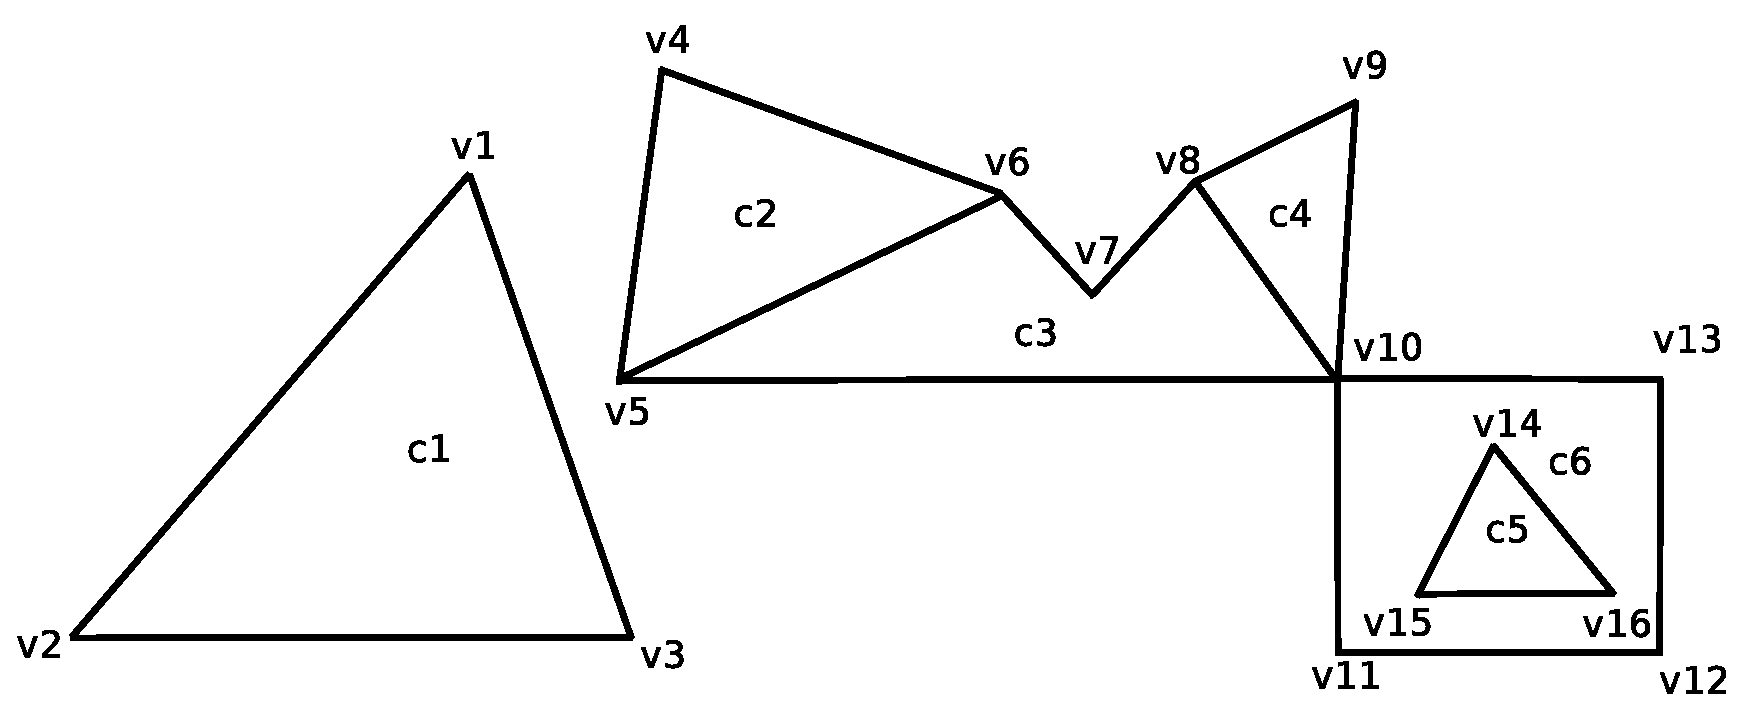
\includegraphics[width=10cm]{chap02/graph-cycle}\medskip
\caption{图中的环}
\label{fig:graph-cycle}
\end{figure}


检测图中的所有的环的问题,实际上就是检测图中的最小环基的问题。要在图像中检测最小环基,首先应先检测分叉点及其之间的连接关系,根据其连接关系,构造搜索路径,以此来实现检测环的过程。

\subsection{分叉点与连接关系检测}
\label{}

二值图像中,若背景为黑,即其像素值是$0$,线为白,即像素值是$1$。要判断一个像素点是否为分叉点,首先应定位线的位置,即判断像素值是否为$1$,然后判断这个像素点的八邻域像素为$1$的像素个数,若八邻域没有像素为$1$的像素,则认为是度为$1$的顶点,即孤立点,若八邻域有$1$个像素值为$1$的像素,则认为这两个点形成一条短线段,这些点都不认为是分叉点。这样研究对象为八邻域内有大于等于$3$个像素值为$1$的点。通过观察与实验发现若八邻域有$3$个像素值为$1$的像素,则中心点其八邻域像素值为$1$的点形成三分叉,中心点可被认为是三分叉点,如图\ref{fig:FeaturePoints}所示,图(a)中的红色点八邻域内有$3$个值为$1$的点,则红色点为三分叉点。三分叉点的常见情况如图\ref{fig:FeaturePoints-image}(a)所示。

而若某一点的八邻域有三个以上像素值为$1$的像素,则不能单纯的认为是几分叉点,如图\ref{fig:FeaturePoints}(b)所示是四分叉点的例子,红色点及蓝色点八邻域都有$3$个以上的值为$1$的点,但蓝色点不能认为是分叉点。

这种情况下,我们要进行连通区域标记。首先重新定位可能是分叉点的点,即其八邻域有$3$个以上像素值为$1$的点。然后要进行连通区域标记,图\ref{fig:FeaturePoints}(b)中的红色及蓝色点标记为一个区域,根据标记点的坐标,计算连通区域的中心位置,最后把中心位置点作为同一个连通区域的分叉点,而连通区域内的其他点为普通点,即红色点作为连通区域的中心,看作是真正的四分叉点。在图像中\ref{fig:FeaturePoints}(b)显示为\ref{fig:FeaturePoints-image}(b),通过计算,蓝色点为中心位置点,即四分叉点。

\begin{figure}
\centering
  \begin{minipage}[b]{0.48\textwidth} 
      \centering 
      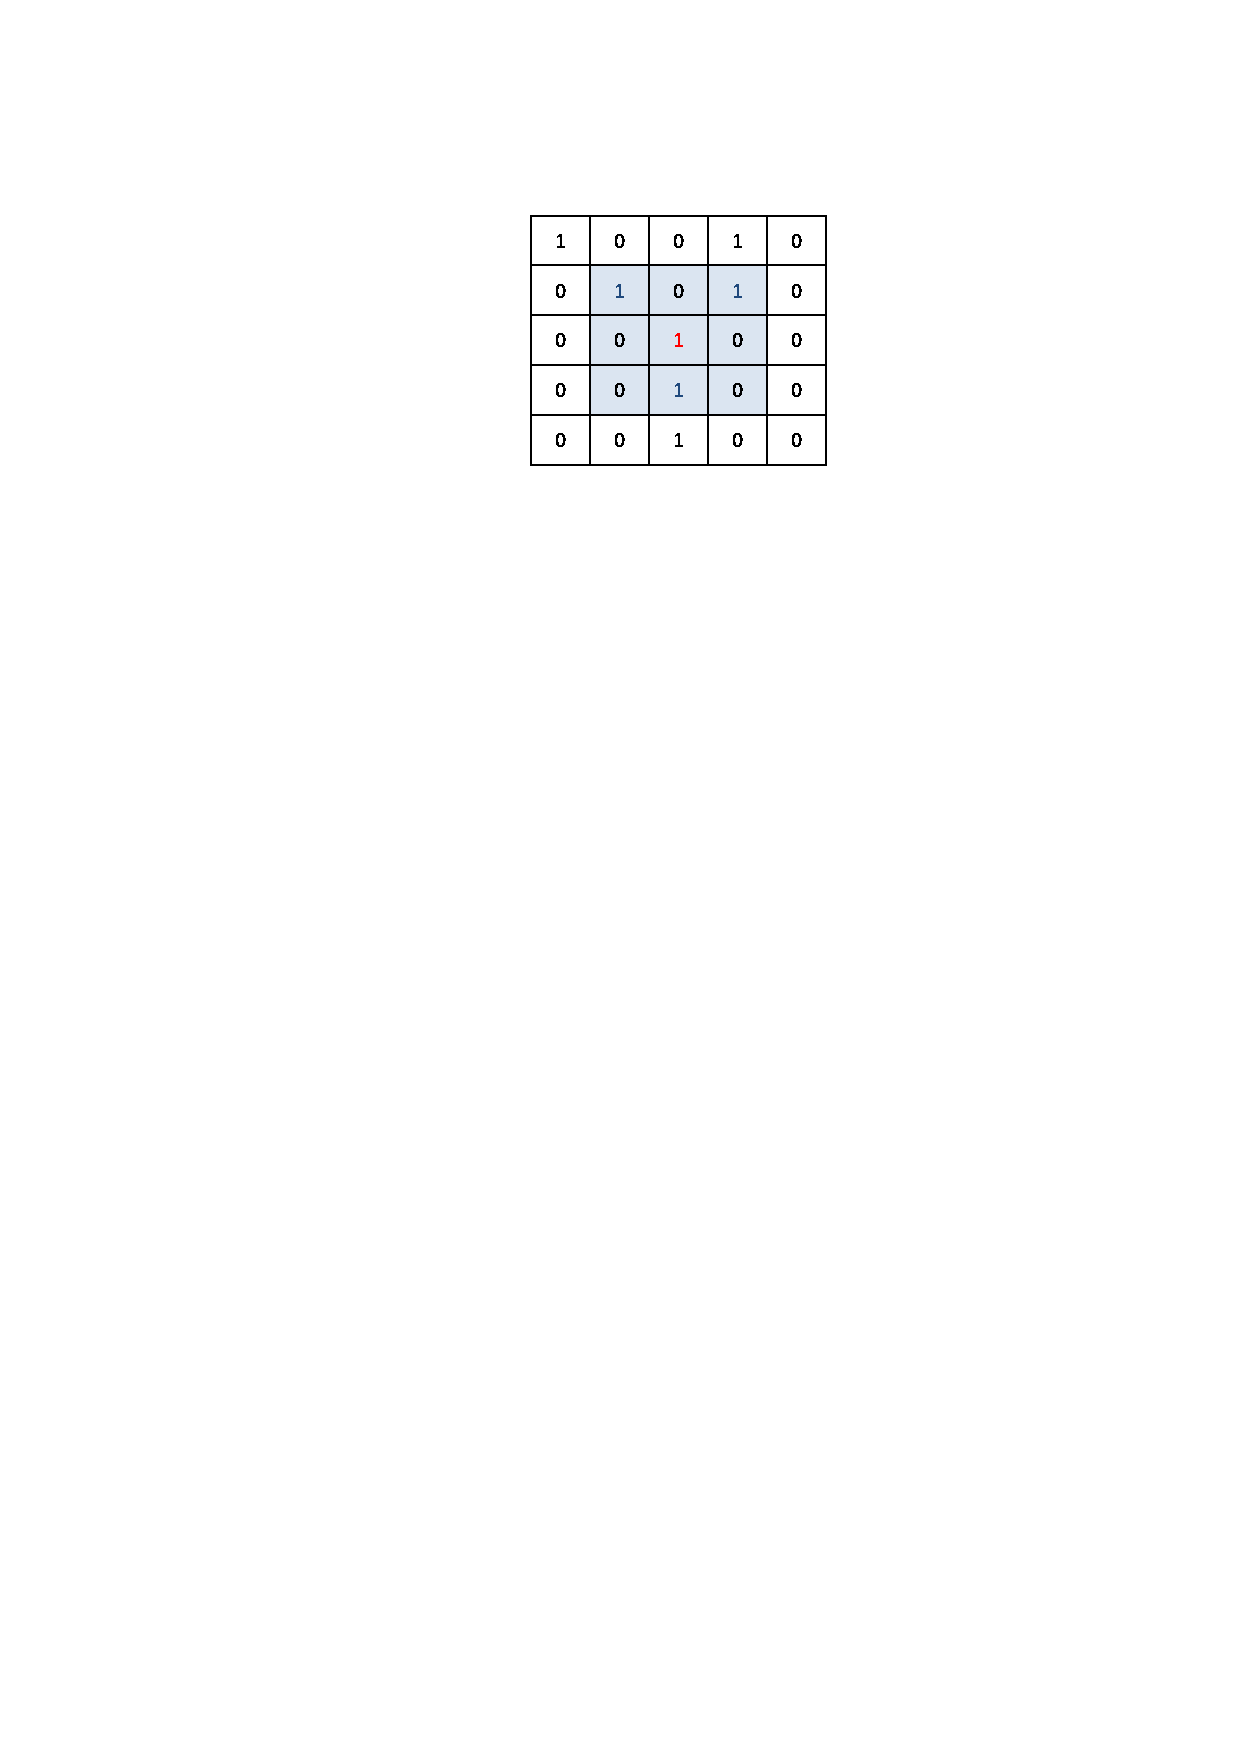
\includegraphics[width=4cm]{chap02/3FeaturePoint}
        \centerline{(a)}\medskip
	 \label{fig:3FeaturePoint}
    \end{minipage}
  \begin{minipage}[b]{0.48\textwidth}
    \centering
    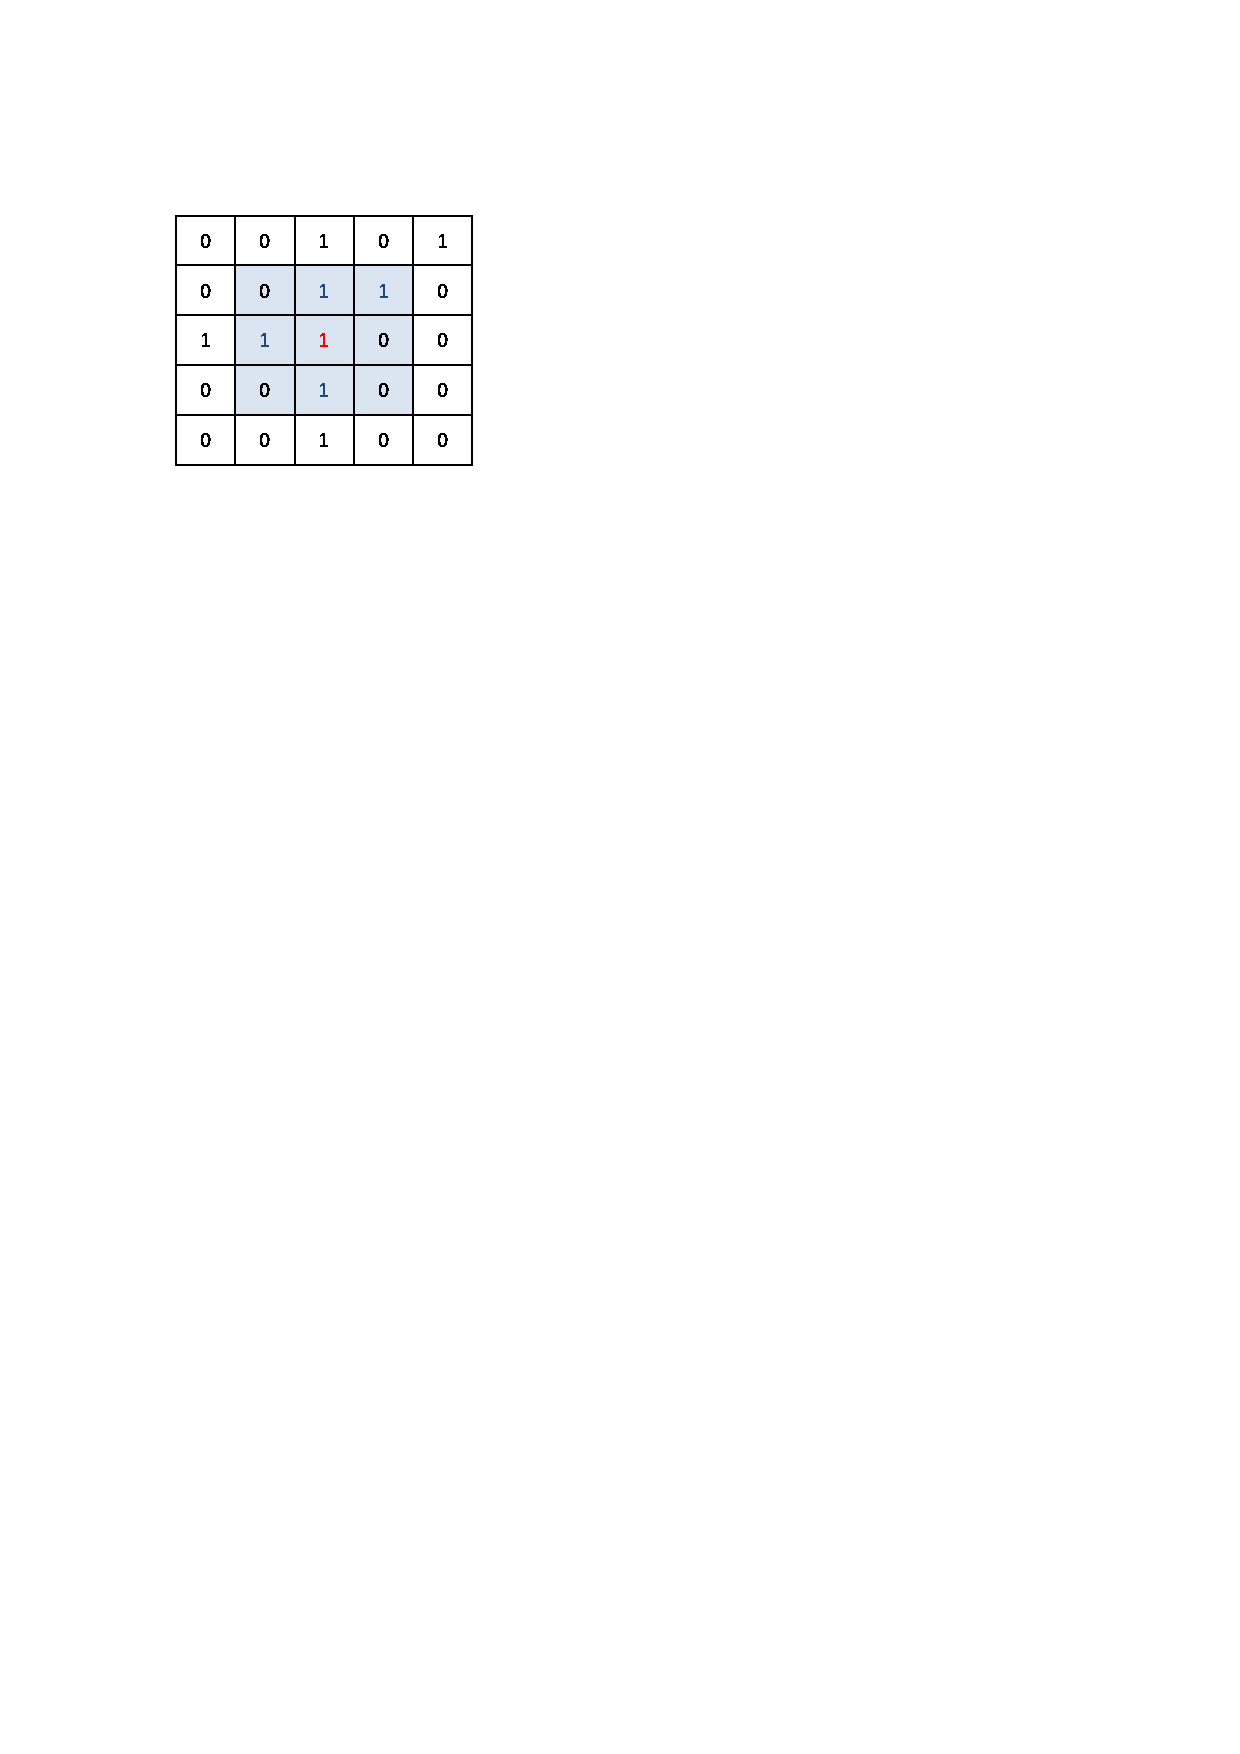
\includegraphics[width=4cm]{chap02/4FeaturePoint}
      \centerline{(b)}\medskip
	\label{fig:4FeaturePoint}
  \end{minipage}
\caption{三分叉点与四分叉点}
\label{fig:FeaturePoints}
\end{figure}

\begin{figure}
\centering
  \begin{minipage}[b]{1\textwidth} 
      \centering 
      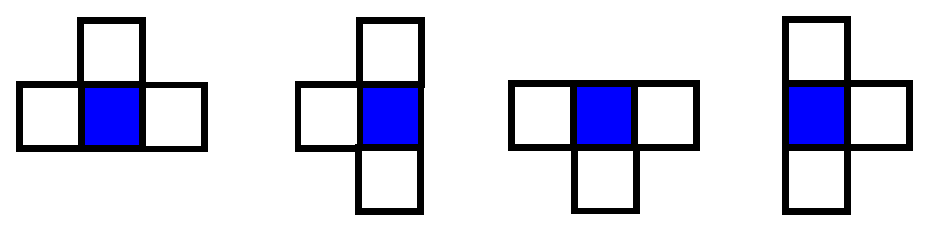
\includegraphics[width=8cm]{chap02/three-bifu}
        \centerline{(a)}\medskip
    \end{minipage}
  \begin{minipage}[b]{1\textwidth}
    \centering
    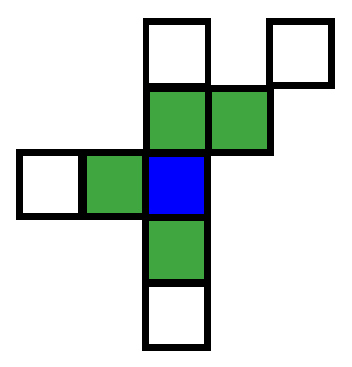
\includegraphics[width=3cm]{chap02/four-bifu}
      \centerline{(b)}\medskip
  \end{minipage}
\caption{三分叉点与四分叉点}
\label{fig:FeaturePoints-image}
\end{figure}

当所有的分叉点都检测到后,每个分叉点被看做一个种子,沿其八邻域像素值为$1$的方向不断向外扩展,直到找到与这个分叉点相邻的分叉点。遍历所有分叉点后,所有的分叉点及其连接关系就被检测到。为了方便后续操作,我们将采用顶点---边矩阵来表示分叉点及其连接关系,于是得到图\ref{fig:graph}的点---边关系表\ref{tab:AdjacentStructure},第一列为所有的分叉点,其余几列为与分叉点相连的分叉点。
\renewcommand\arraystretch{0.8}
\begin{table}[H]
\caption{点---边关系}
\centering
\begin{tabular}{p{2cm}<{\centering}p{1cm}<{\centering}p{1cm}<{\centering}p{1cm}<{\centering}}
  \hline
  分叉点 & \multicolumn{3}{c}{相邻分叉点}\\
  \hline
  \rowcolor{gray!50}
  $v_{1}$ & $v_{2}$  & $0$      & $0$  \\
  $v_{2}$ & $v_{1}$  & $v_{3}$  & $v_{4}$ \\
  \rowcolor{gray!50}
  $v_{3}$ & $v_{2}$  & $v_{4}$  & $0$\\
  $v_{4}$ & $v_{2}$  & $v_{3}$  & $0$ \\
  \rowcolor{gray!50}
  $v_{5}$ & $0$      & $0$      & $0$\\
  \hline
\end{tabular}
\label{tab:AdjacentStructure}
\end{table}

众所周知,能够组成环结构的分叉点数目至少为$3$,这就要求每个分叉点的度大于等于$3$,即$d_{v_i} \geq 3$,并且每个分叉点应至少在点---边关系矩阵中出现$3$次。通过这个规则,可以滤除一些不能组成环结构的点。但这个过程不能一次滤除所有的不能组成环结构的无效点,而是需要进行循环滤除,每进行一次,最外围的无效点将会滤除,直到所有的无效点被滤除后,循环得以结束。以一个视网膜图像为例,如图\ref{fig:Bifurcation},分别表示初始检测到的分叉点与所有无效分叉点被滤除后的图像,从图中可以看出,分支末端的点都被滤除,只剩下可能组成环的分叉点。通过滤除不能组成环的无效的分叉点,就可以大大的减少搜索环的路径,从而减小环检索算法的复杂度。

\begin{figure}
\centering
  \begin{minipage}[b]{0.48\textwidth} 
      \centering 
      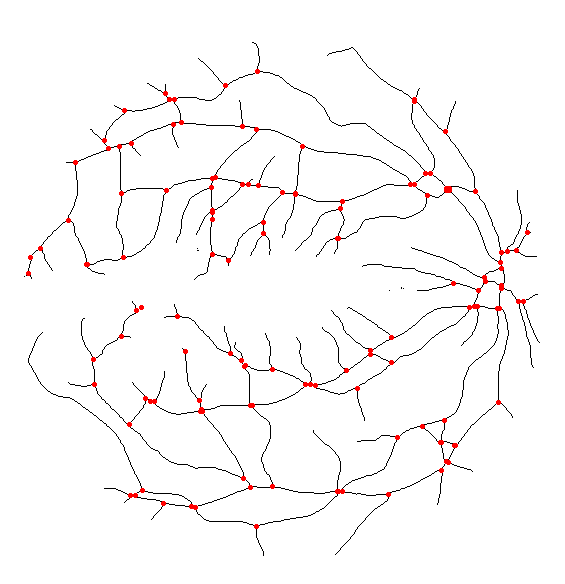
\includegraphics[width=4cm]{chap02/all-bifu}
        \centerline{(a)所有分叉点}\medskip
	 \label{fig:3FeaturePoint}
    \end{minipage}
  \begin{minipage}[b]{0.48\textwidth}
    \centering
    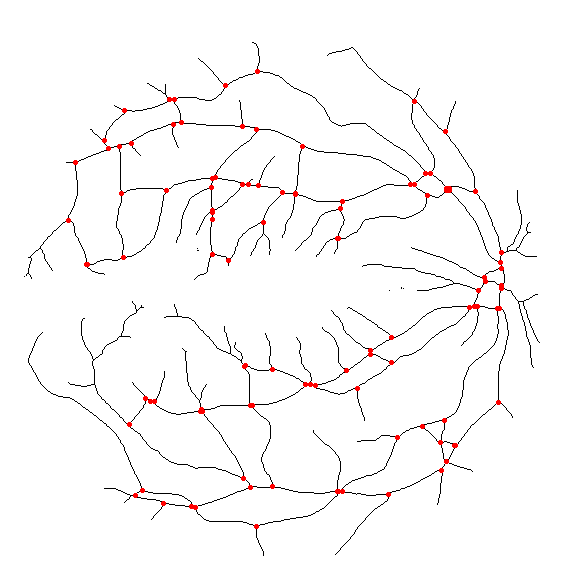
\includegraphics[width=4cm]{chap02/select-bifu}
      \centerline{(b) 可能组成环的分叉点}\medskip
	\label{fig:4FeaturePoint}
  \end{minipage}
\caption{所有分叉点与滤除无效分叉点后的对比图}
\label{fig:Bifurcation}
\end{figure}

\subsection{基于广度优先策略的环结构检测}
\label{}


在图中检测最小环基的问题实际上是图论中的一个被广泛研究的问题。Joe Kirk 提出了迭代环计数算法,算法的基本思想是通过动态路径搜索环,动态路径实际上是把图变换成一棵树,路径表示树上的一个结点到另一个结点的连线,当一个节点在一条路径上出现两次,则表示这条路径上的点形成一个环。

树的定义如下:
树是包括n个结点的有限集合$T(n \geq 1)$~\cite{zhangming},使得
\begin{enumerate}
\item 有且只有一个特定的成为根的结点。
\item 除根以外的其他结点被分成m个$(m \geq 0)$个不相交的有限集合$T_1, T_2, \ldots, T_m$,而每一个集合又都是树。其中,树$T_1, T_2, \ldots, T_m$称作这个根的子树。
\end{enumerate}

这个定义是递归的,即在树的定义中又用到了树的概念。在一棵树中,若存在节点$k$指点个结点$k'$的连线,则称$k$是$k'$的父结点,而$k'$是$k$的子结点,有向连线$<k, k'>$称作边。同一个父结点的子结点之间称为兄弟。树中没有父结点的结点称为根,没有子结点的结点称为树叶。若树中存在结点序列$k_0,k_1,\ldots,k_s$,使得$<k_0,k_1>,<k_1,k_2>,\ldots,<k_{s-1},k_s>$都是树中的边,则称从结点$k_0$到结点$k_s$存在一条路径。若有一条由$k$到达$k_s$的路径,则称$k$是$k_s$的祖先,$k_s$是$k$的子孙。图\ref{fig:tree}表示一棵树,$A$表示根结点,$B$、$C$是$A$的子结点,$A$是$BC$的父结点,$BC$为兄弟结点。$ABDI$是一条路径,其中$A$是$I$的祖先,$I$为$A$的子孙。

\begin{figure}
\centering
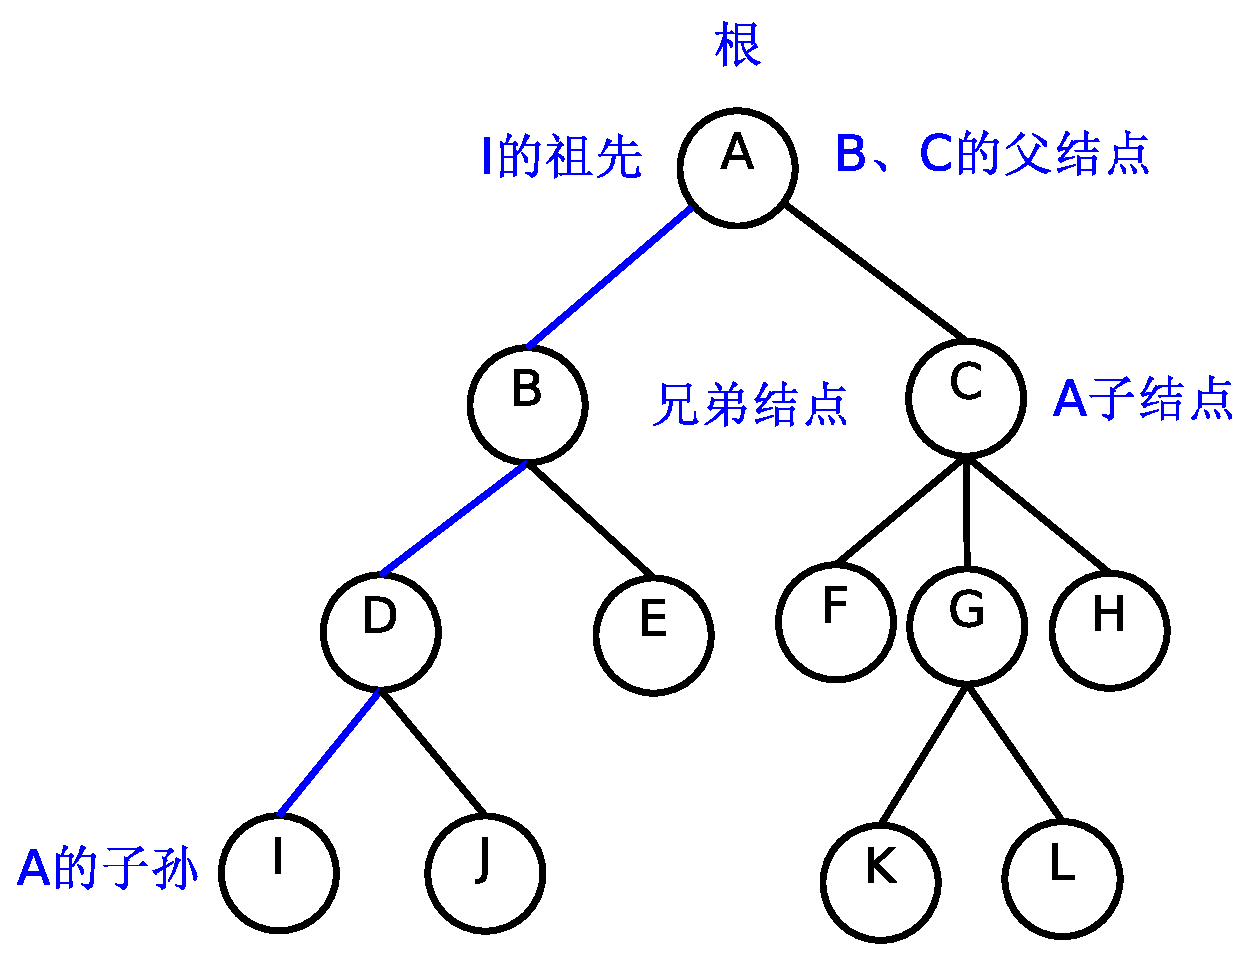
\includegraphics[width=0.5\textwidth]{chap02/tree-1}
\caption{树形表示法}
\label{fig:tree}
\end{figure}

在树中顺序搜索结点叫做树的遍历。通常有两种遍历方法:深度优先遍历与广度优先遍历。
\begin{itemize}

\item 深度优先遍历算法。深度优先算法的思想是尽可能沿分支结点向深度方向进行遍历。对于二叉树来说,深度优先即先沿着分支结点向左下降,当遇到左子树为空的时候,返回到上面最近的且其右子树尚未访问到的分支结点,转向该分支节点的右子结点,然后再尽可能地沿着左链前进。重复执行上述过程,直到遍历完所有的结点为止。

进行深度优先遍历时,结点既可以在向下遍历之前访问,也可以在从子树返回之后访问,根据结点的访问时间,可以定义不同的深度优先遍历算法,即前序法、中序法、后序法。前序法即先访问根结点,然后访问左子树,最后访问右子树。中序法先访问左子树,然后访问根结点,最后访问右子树。而后序法首先访问左子树,然后访问右子树,最后访问根结点。如图\ref{fig:dfs}所示为一个图,按前序法进行深度优先遍历时,访问结点的顺序应该是$ABDECFG$。

\item 广度优先遍历算法。广度优先又叫宽度优先或横向优先,是从上而下,从左到右地按层次进行遍历。其过程是:首先访问树的第一层,即根结点所在的层,然后从左到右依次访问第二层的结点,依次类推,当第$i$层的所有结点访问结束后,再从左到右依次访问第$i+1$层的各个结点。图\ref{fig:dfs}进行广度优先搜索的结果为$ABCDEFG$。

\end{itemize}

\begin{figure}[H]
\centering
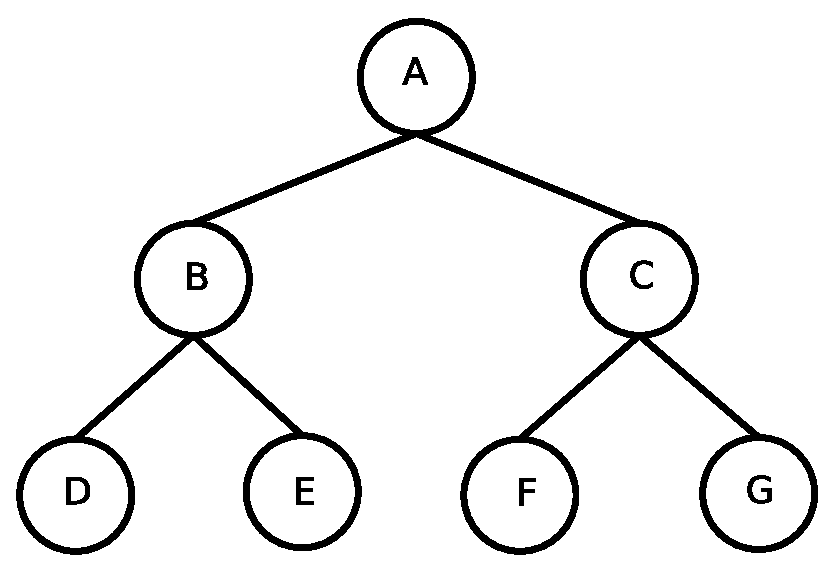
\includegraphics[width=0.4\textwidth]{chap02/dfs}
\caption{深度优先与广度优先}
\label{fig:dfs}
\end{figure}

迭代环计数算法也依赖于点---边关系矩阵,该算法利用了深度优先算法的思想,主要步骤为:
\begin{enumerate}
\item 初始化一个结点作为树的根。
\item 找到与这个结点相邻的结点,并把其中一个结点作为根的子结点,放入树的第二层。
\item 继续找与第二层中的点相邻的一个结点,作为树的第三层。在搜索根的子结点的相邻点的过程中,要排除其上一层中的点,即根结点不作为树的第三层中的点。
\item 若路径中包含两个相同的结点,则说明这个路径中的结点形成一个环,并继续按照点边关系寻找下一个结点。
\item 若没有环形成,则继续寻找下一个结点,并更新路径。
\item 若这条路径已经到最后一个结点,则回到树的上一层并更新路径。
\item 重复$2$到$6$步直到第$8$步完成。
\item 如果当前结点不是第一个结点,并且所有的结点都已搜索到则算法结束。
\end{enumerate}

如图\ref{fig:graph-tree},a表示一个图,b是根据迭代环计数算法转换成的树。首先初始化一个点$1$作为树的根,根据点边关系矩阵,搜索到$1$的子结点$2$,放入树的第二层,根据$2$的点边关系矩阵,搜索到$3$结点,放入树的第三层,继续搜索$3$的点边关系矩阵,得到结点$1$,此时结点$1$、$2$、$3$、$1$形成一个环结构,然后回溯到$1$的上一层,即第三层继续寻找除$1$以外与$3$相连的其他点,即$4$点,然后继续搜索,直到遍历所有的点边关系矩阵。由此,遍历结束后,得到三个环结构,即$123$、$1243$、$243$。重复搜索的环将在遍历结束后被去除。
\begin{figure}[H]
\centering
  \begin{minipage}[b]{0.48\textwidth} 
      \centering 
      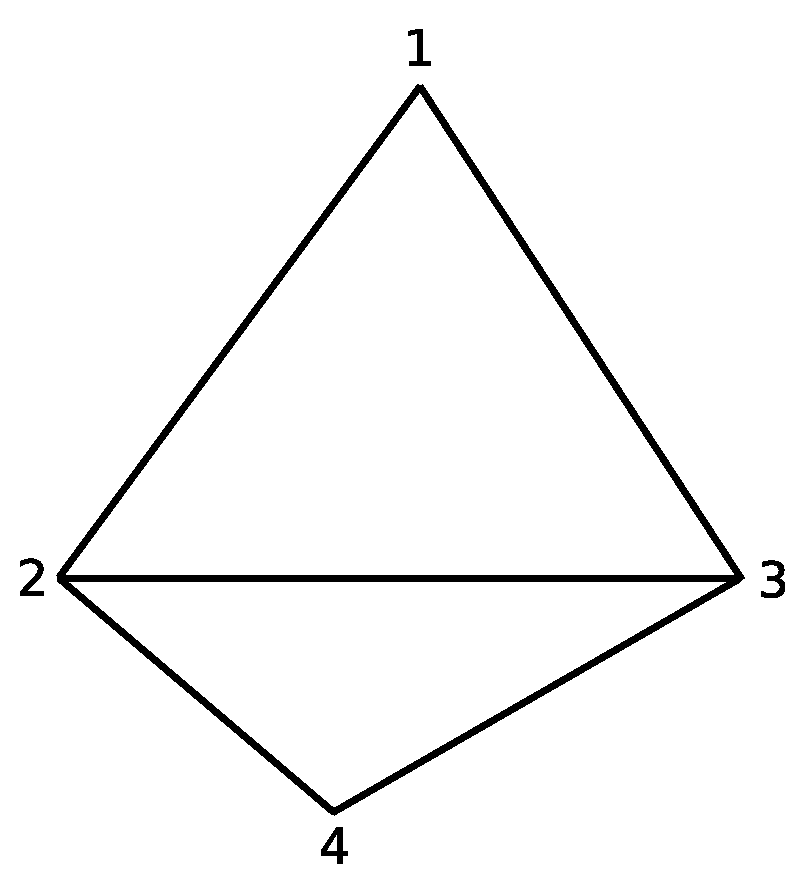
\includegraphics[width=4cm]{chap02/loop}
        \centerline{(a)图}\medskip
    \end{minipage}
  \begin{minipage}[b]{0.48\textwidth}
    \centering
    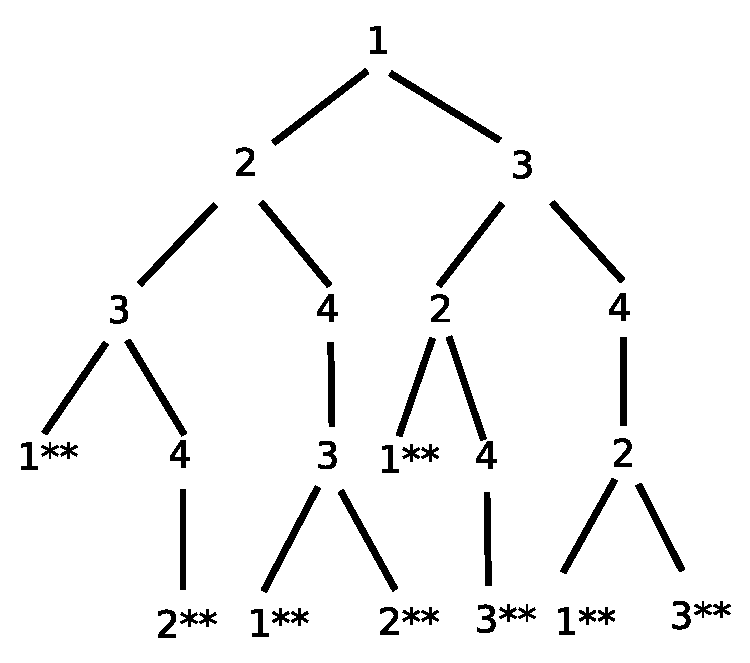
\includegraphics[width=5cm]{chap02/graph-old}
      \centerline{(b) 树}\medskip
  \end{minipage}
\caption{图与迭代环计数算法转化树}
\label{fig:graph-tree}
\end{figure}

由此可知,迭代环计数算法能够检测到图中的所有环,不仅包括最小环,还存在由最小环形成的大环。在图像中,我们感兴趣的是提取图像中的最小环结构。并且当图像中的环结构较多,点边关系错综复杂时,深度优先算法的搜索路径往往容易变得冗长,且迭代环计数算法的搜索路径容易重复,从而增加算法复杂性。

基于此,我们提出了基于广度优先检索策略的环结构检测算法,使得树结构更加简单,从而减小算法的复杂性。算法思想同样是把图变换成一颗树,但是基于广度优先算法,并且增加了对于兄弟结点的考虑,从而降低算法的复杂性,其主要步骤为:
\begin{enumerate}
\item 初始化一个结点作为树的根。
\item 找到与这个结点相邻的所有结点,并把他们作为根的子结点,放入树的第二层。相邻的点可以通过点边邻接矩阵得到,因为它列出了与某一点相邻的所有的结点。
\item 判断当前层是否有相邻的兄弟结点或相同的结点,若有,则说明有环形成。回到上一层,找到其相同的父结点或相邻的不同的父结点,若没有找到,则继续回到上一层,直到找到为止,那么,搜索路径上的点就可以组成环。
\item 继续检测与当前层的结点相连的除父结点及兄弟结点以外的其他结点并放入树的下一层。然后转入第三步,直到所有的点边关系遍历结束。
\end{enumerate}
经过以上步骤,所有三点、四点、五点环将被检测到。如图\ref{fig:cycle-tree}(a)是一个图的例子,图中有一个三点环、一个四点环、一个五点环。通过我们的环结构检测算法,这三个环要被准确无误的检测出来。首先确定$v_1$为初始点,即树的根。通过点边关系可得,与之相邻的点分别为$v_2, v_5, v_6, v_8$,于是,这四个点将被当作根的子结点放入树的第二层。判断这四个点是否有相邻点,发现$v_5, v_6$是相邻的,那么$v_5, v_6$及其相同的父结点$v_1$形成一个三点环,继续寻找这四个点的相邻点(除父结点及兄弟结点以外),放入树的第三层。判断这些点有没有相邻点或相同点。通过点边关系矩阵发现$v_3,v_4$是相邻点,那么$v_3,v_4$与其父结点$v_2,v_5$及其父结点的相同父结点$v_1$形成五点环,同理,$v_{1}v_{6}v_{7}v_{8}$组成四点环。至此,所有的搜索都已完成,即共找到三个环,$v_{1}v_{5}v_{6}$组成三点环,$v_{1}v_{6}v_{7}v_{8}$组成四点环,$v_{1}v_{2}v_{3}v_{4}v_{5}$组成五点环。

\begin{figure}
\centering
  \begin{minipage}[b]{1\textwidth} 
      \centering 
       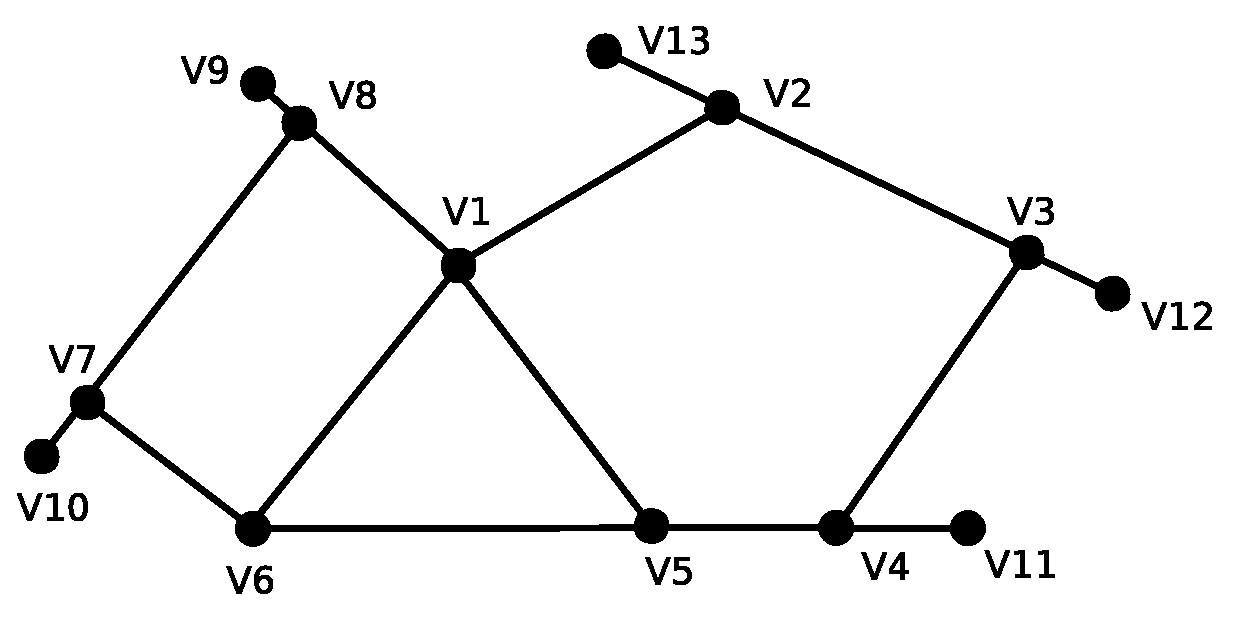
\includegraphics[width=7cm]{chap02/graph2}
       \centerline{(a)}\medskip
    \end{minipage}
  \begin{minipage}[b]{1\textwidth}
    \centering
    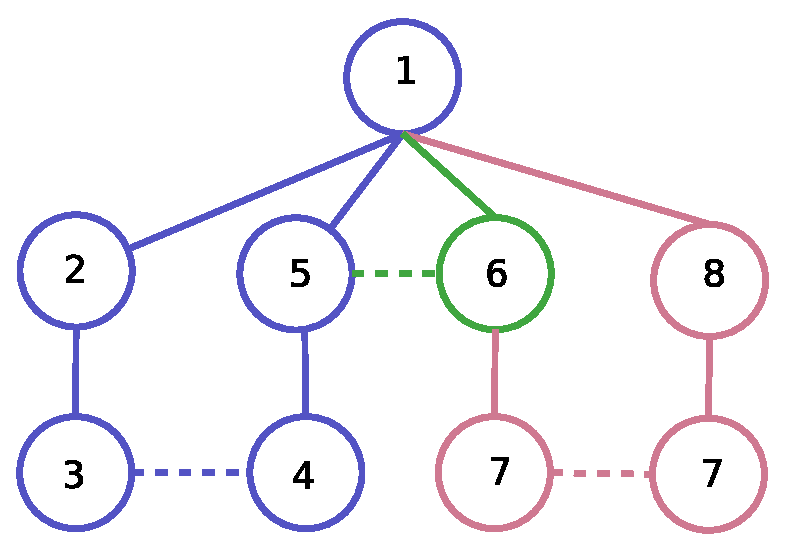
\includegraphics[width=6cm]{chap02/tree}
    \centerline{(b)}\medskip
  \end{minipage}
\caption{图与搜索树}
\label{fig:cycle-tree}
\end{figure}

通过我们提出的环结构检测算法算法,图\ref{fig:graph-tree}(a)可以转化为图\ref{fig:simple-tree}中的树,由此可以看到,相比图\ref{fig:graph-tree}(b)中的树,图\ref{fig:simple-tree}更加的简单,搜索路径不会重复,算法更加高效。

\begin{figure}
\centering
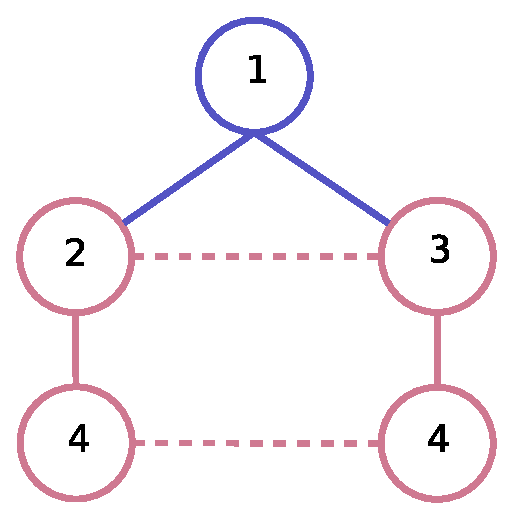
\includegraphics[width=0.3\textwidth]{chap02/simple-graph}
\caption{图\ref{fig:graph-tree}(a)的搜索树}
\label{fig:simple-tree}
\end{figure}


\section{环结构描述}
\label{}
环之所以能用在图像识别与匹配领域,是因为它是稳定的显著的特性。而它的稳定性与显著性则体现在用来描述环结构的特征向量上。

一个环结构是由一系列分叉点与连接这些分叉点之间的线组成。我们用分支角度与分支长度来描述环结构。以任意分叉点$v_i(x_0, y_0)$为中心,构造一个$7 \times 7$的邻域。记录分支与邻域边缘$24$个像素相交点的坐标,假设其坐标值为$x_j, y_j, j=1, 2, \ldots$。则分支方向为:
\begin{align}
\beta_j = arctan\frac{dy}{dx}, dy = y_j - y_0, dx = x_j - x_0 
\end{align}

由于$arctan$的取值范围为$-90^{\circ} \sim 90^{\circ}$,故还需保证求出的角度大于$0$。即
\begin{align}
\alpha_j = \left\{ \begin{array}{ll}
\beta_j & \textrm{$dy \geq 0$, $dx \geq 0$} \\
\beta_j + 180^{\circ} & \textrm{$dy \geq 0$, $dx \leq 0$ 或 $dy \leq 0$, $dx \geq 0$}\\
\beta_j + 360^{\circ} & \textrm{$dy \leq 0, dx \leq 0$}
\end{array} \right.
\end{align}

邻域边缘$24$个像素把$360^{\circ}$分成了$24$个离散值,每个相邻的分支角度相差$15^{\circ}$。每个角度以水平线为基准,故分叉点之间的角度值可通过式\ref{eq:Angle}计算:
\begin{align}
\theta_i = \alpha_{i+1} - \alpha_i, \qquad
\theta_i = \left\{ \begin{array}{ll}
\theta_i + 360^{\circ} & \theta_i \le 0 \\
\theta_i & \theta_i \geq 0
\end{array} \right.
\label{eq:Angle}
\end{align}

如图\ref{fig:calculate-angles},以三分叉点为中心划定一个$7\times7$邻域,邻域的边缘$24$个像素把$360^{\circ}$分为$24$个方向的角度,分别为$15^{\circ}, 30^{\circ},45^{\circ}, \ldots, 360^{\circ}$。在这个邻域的边缘$24$个像素中,像素值为$1$的像素以水平线为基准与中心像素形成分支角度,图\ref{fig:calculate-angles}中,共形成$3$个角度,即$45^{\circ}, 150^{\circ},270^{\circ}$,则分支之间的角度为$105^{\circ}, 120^{\circ}, 135^{\circ}$。

\begin{figure}[H]
\centering
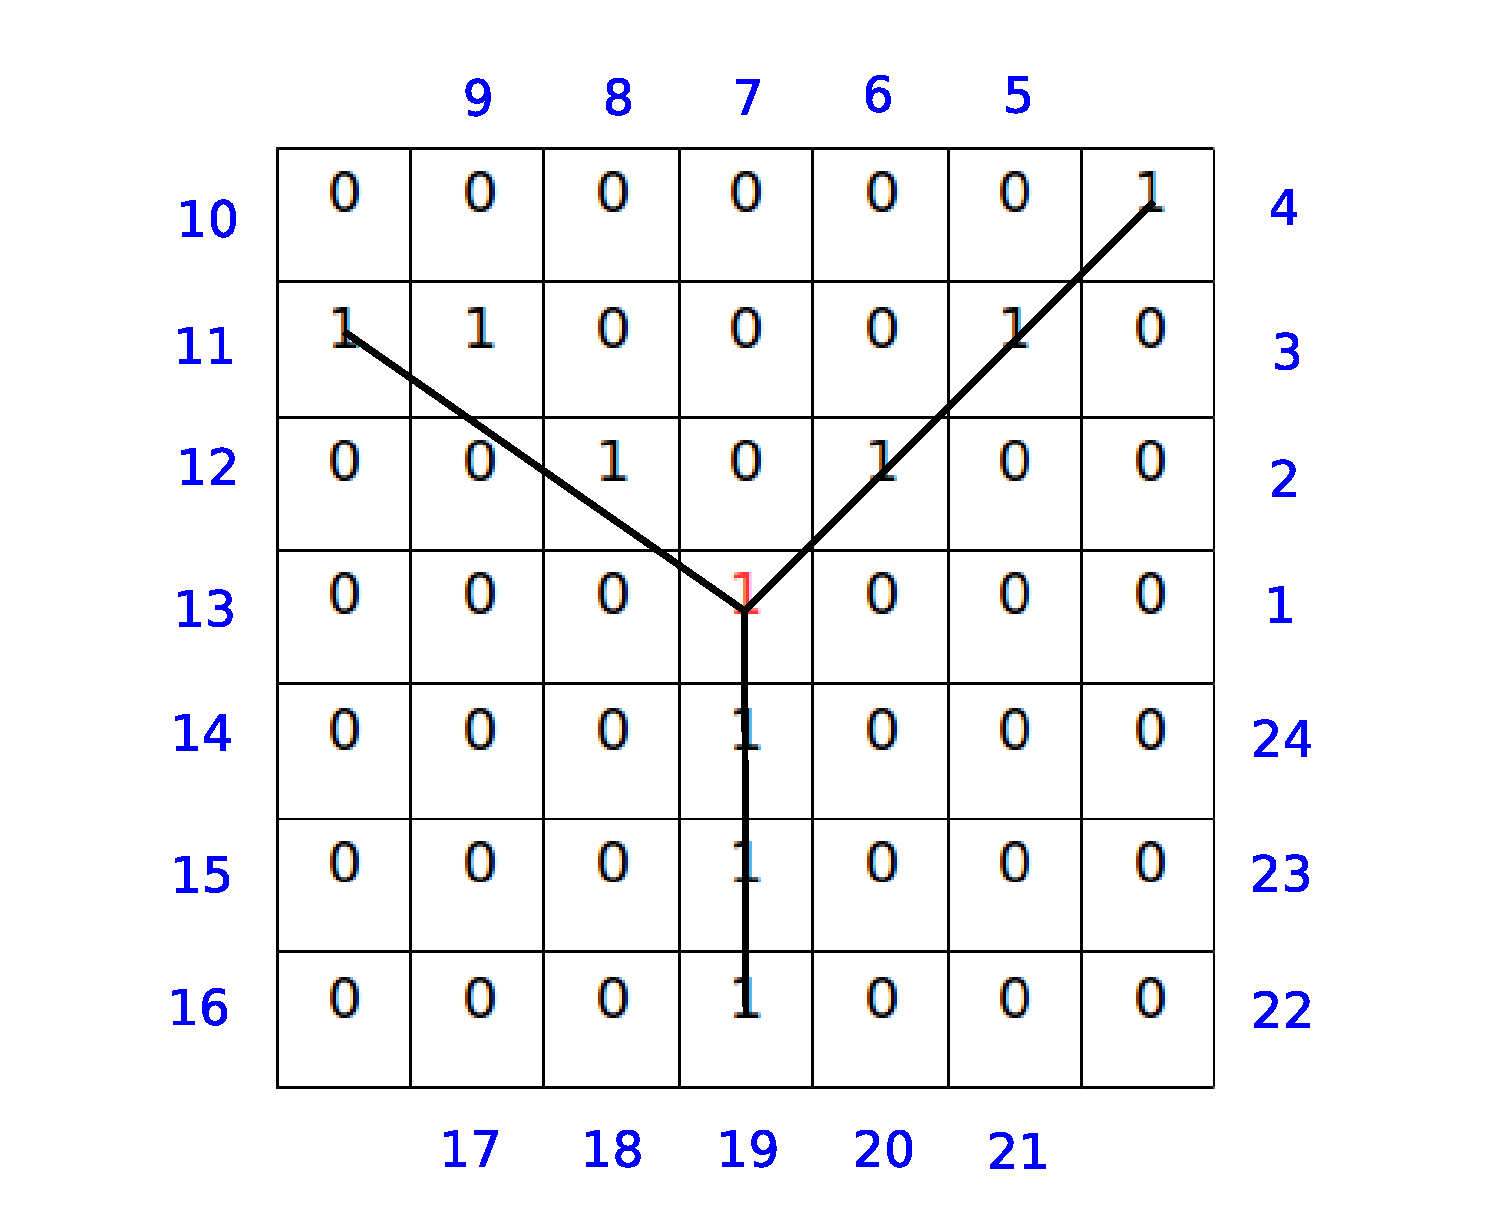
\includegraphics[width=0.5\textwidth]{chap02/7-7}
\caption{分支角度计算}
\label{fig:calculate-angles}
\end{figure}

分叉点之间的分支长度为分叉点之间的欧式距离,即:
\begin{align}
L = \sqrt{(y_j - y_0)^2 + (x_j - x_0)^2}, j = 1, 2, \ldots
\end{align}

归一化属于数字信号处理范畴,即将有量纲的表达式,经过变换,转换为无量纲的表达式,成为标量。它是简化计算,缩小量值的有效办法。而对于环结构特征,通过归一化,能使在减少计算量的基础上,使环结构特征具有平移、旋转及尺度不变性。图\ref{fig:description}给出了四点环结构示意图,角度归一化、长度归一化及最终产生的特征向量可分别用式\ref{eq:angle}、式\ref{eq:length}及式\ref{eq:vector}表示。$L_{1} \sim L_{4}$,$\theta_{1} \sim \theta_{14}$,$\theta_{15} \sim \theta_{18}$ 分别代表分支长度、分支角度及分叉点之间的角度。

\begin{figure}[H]
\centering
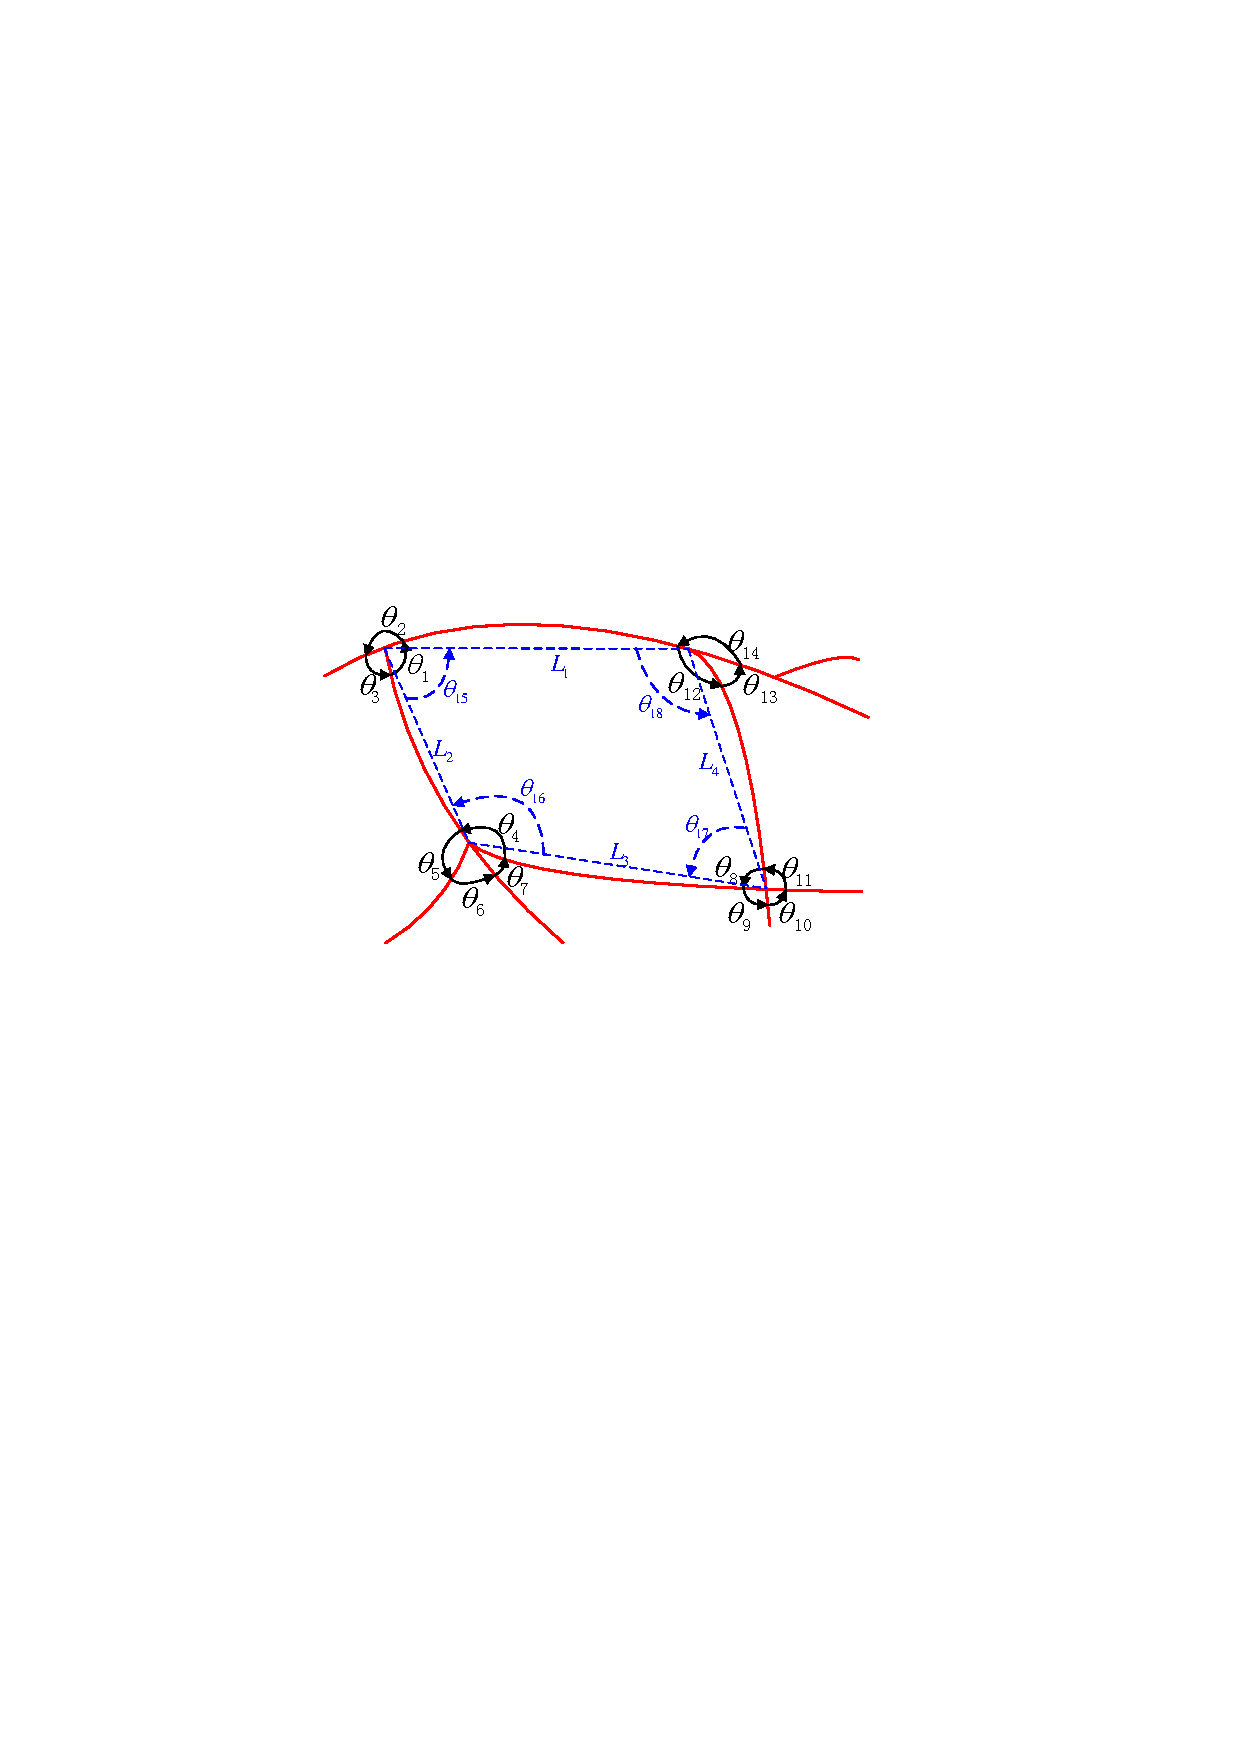
\includegraphics[width=0.4\textwidth]{chap02/description.pdf}
\caption{环结构描述}
\label{fig:description}
\end{figure}
\begin{align}
L_{iNorm}&=\frac{L_i}{\sum{L}}\label{eq:length}\\
\theta_{jNorm}&=\frac{\theta_j}{360^\circ}\label{eq:angle}
\end{align}
\begin{multline}
\tilde{v}=\{\textrm{长度,角度}\}=\{L_{1},L_{2},L_{3},L_{4},\theta_{1},\theta_{2},\theta_{3},\mathbf{0},\theta_{4},\\\theta_{5},\theta_{6},\theta_{7},\theta_{8},\theta_{9},\theta_{10},\theta_{11},\theta_{12},\theta_{13},\theta_{14},\mathbf{0},\theta_{15},\theta_{16},\theta_{17},\theta_{18}\}
\label{eq:vector}
\end{multline}

值得注意的是,组成环的分叉点个数不一样,并且每个分叉点的分叉角度也不同,这就导致了不同类型的环有不同长度的特征向量。为了便于识别和配准的需要,我们可根据实际情况设定一个角度个数标准,比如说,若设置$4$个分支角度为标准,那么小于$4$个角度的分叉应用$0$来补齐,这样就保证同种类型的环的特征向量的长度是相同的。这样,当用来做配准或识别时,就可匹配同种类型的环的特征向量来达到目的。

\section{本章小节}
\label{}

本章介绍了环结构特征的定义、特点及应用,阐述了从图像中检测环的主要步骤:检测分叉点及其连接关系、滤除无效分叉点、检测环结构,并重点介绍了我们提出的环结构检测算法。同时,结合环结构的特点,给出了特征描述的方法。通过把环结构特征表示成为特征向量,就能为下一步的配准、识别奠定基础。
